\documentclass[UTF8, a4paper, 12pt, fontset=fandol]{ctexart}

\usepackage[margin=2.6cm]{geometry}
\usepackage{setspace}
\setstretch{1.5}
\setlength{\parskip}{0.4em}
\setlength{\parindent}{2em}

\usepackage{amsmath}
\usepackage{amssymb}
\usepackage{mathtools}
\usepackage{amsthm}
\usepackage{bm}
\usepackage{latexsym}
\usepackage{array}
\usepackage{booktabs}
\usepackage{dcolumn}
\usepackage{multirow}
\usepackage{makecell}
\usepackage{tabularx}
\usepackage{threeparttable}
\usepackage{longtable}
\usepackage{siunitx}
\usepackage{graphicx}
\usepackage{float}
\usepackage{subcaption}
\usepackage{caption}
\usepackage{enumitem}
\usepackage{xcolor}
\usepackage{microtype}
\usepackage{csquotes}
\usepackage{listings}
\usepackage{algorithm}
\usepackage{algpseudocode}
\usepackage{fancyhdr}
\usepackage{hyperref}
\usepackage[nameinlink]{cleveref}
\usepackage[numbers,sort&compress,square]{natbib}
\usepackage{appendix}
\usepackage{lmodern}

\hypersetup{
  colorlinks=true,
  linkcolor=blue,
  citecolor=blue,
  urlcolor=blue
}

\lstset{
  basicstyle=\ttfamily\small,
  numbers=left,
  numberstyle=\tiny,
  frame=single,
  breaklines=true,
  keywordstyle=\color{blue},
  commentstyle=\color{gray}
}

\newtheorem{theorem}{定理}[section]
\newtheorem{lemma}[theorem]{引理}
\newtheorem{proposition}[theorem]{命题}
\theoremstyle{definition}
\newtheorem{definition}{定义}[section]
\newtheorem{assumption}{假设}[section]
\theoremstyle{remark}
\newtheorem*{remark}{注记}

\newcommand{\E}{\mathbb{E}}
\newcommand{\Prb}{\mathbb{P}}
\newcommand{\Var}{\operatorname{Var}}
\newcommand{\Cov}{\operatorname{Cov}}
\newcommand{\indep}{\mathop{\perp\!\!\!\perp}}
\newcommand{\ind}[1]{\mathbf{1}(#1)}

\pagestyle{fancy}
\fancyhf{}
\fancyfoot[C]{\thepage}
\fancyhead[L]{生成式人工智能与内容平台动态治理}
\setlength{\headheight}{14.5pt}

\title{生成式人工智能与内容平台的动态治理：从普惠式扩量到选择性扶持}
\author{朱千子 \quad 朱胜豪\\[0.5em]\small 对外经济贸易大学经济学院}
\date{\today}

\begin{document}

\maketitle

\begin{abstract}
本文研究生成式人工智能降低数字内容生产成本以后，内容平台为何可能从普惠式项目
扶持转向选择性准入与绩效激励，并以AI短剧作为主要应用场景。模型包含平台、
异质创作者和稀缺的用户注意力。
平台在每一期先公布固定支付与收入分成，创作者据此决定是否进入并选择不可合同化的
质量努力，平台在观察内容后再配置推荐曝光。更多项目进入一方面扩大题材和团队的
试验范围，另一方面造成注意力拥堵、筛选成本和创作者激励稀释。
本文首先求解终端期的曝光、努力和进入均衡；随后建立$t\in\{1,2\}$的两期
离散时间模型，引入创作资本与推荐资本的跨期积累；最后给出离散时间无限期
Bellman方程，并在扩展模型中以项目反馈构造贝叶斯后验状态和受控马尔可夫转移。
全文的核心对象是项目进入的动态边际价值：它等于当期边际利润、
创作资本积累价值与推荐学习价值之和。该边际价值在零补贴自然进入规模处的符号，
统一决定平台应当扩大补贴、维持零补贴还是使用选择性准入。模型表明，当推荐资本
逐步成熟、数据学习的边际价值下降而自然进入规模上升时，存在一个内生的技术成熟
阈值；跨过该阈值以后，统一非负补贴不能实施平台的目标进入规模，政策因而从普惠
式扩量转向资格审核、项目申请制和定向扶持。本文进一步在统一的期内均衡原语下，
用向后归纳求解两期均衡，并用值函数迭代求解无限期平稳马尔可夫均衡。类别多样性
由公开短视频数据约束，其余参数作为透明的部分校准并接受网格与参数敏感性检验。
数值均衡复现了早期正支持、成熟期零支付配额的转换。该转换依赖于学习收益相对于
当期匹配改善收益的下降速度，并非
由技术进步机械推出。随机扩展进一步表明，当平台对潜在匹配状态的后验精度可以由
新增项目反馈内生提高且信息边际价值递减时，确定性成熟阈值可推广为依赖创作资本
与后验均值的精度阈值。
\end{abstract}

\begin{center}
\textbf{关键词：} 生成式人工智能；内容平台；平台治理；注意力拥堵；动态合同；推荐资本；贝叶斯学习
\end{center}

\section{引言}
\label{sec:intro}

生成式人工智能正在改变数字内容市场的主要稀缺性：剧本、图像、声音和视频片段的
生成成本下降以后，稀缺资源逐步从“谁有能力生产”转向“哪些内容值得被发现、精修
和分配注意力”。任务方法的宏观研究强调，人工智能的经济作用首先体现为特定任务的
成本节约或互补性改善，不能由模型能力直接推断总体价值\citep{acemoglu2025simpleai}。
企业场景的微观证据则表明，生成式人工智能可以提高平均生产率并使经验较少的劳动者
受益更多，但效果具有明显的任务与技能异质性\citep{brynjolfsson2025genaiwork}。
在创意写作实验中，人工智能建议提高了单个作品的平均评价，却也使作品之间更为相似
\citep{doshi2024creativity}。这些证据并不直接等同于AI短剧市场的均衡效应，但共同
支持本文的出发点：生产成本下降可能同时带来进入扩张、质量改善和内容同质化，而
供给扩张本身并不保证平台价值同比增加。

本文研究的上位对象是“生成式内容平台”，即同时具备异质创作者进入、算法化内容
分发、有限用户注意力以及补贴或收入分成工具的平台。AI短剧是全文的主要应用场景：
它集中体现了剧本、分镜、角色、配音和后期等多项任务被生成式人工智能重组，也高度
依赖平台的冷启动测试和后续推荐。相同机制还可以用于AI漫剧、数字人视频和其他
AI辅助视听内容；但本文不研究基础模型之间的竞争、全经济的就业替代或不依赖推荐
分发的一般创意产业。换言之，AI短剧是识别机制的场景，而不是理论适用性的唯一边界。

内容平台具有典型的多边结构：平台连接创作者、用户以及可能存在的广告主，并通过
合同和治理规则影响各侧参与及其交互\citep{rochet2003platform,hagiu2015multisided}。
创作者经济研究表明，收入分成、创作者支持工具和平台基础设施会共同改变内容供给、
进入构成和生态集中度\citep{bhargava2022creator}。平台的作用也不限于定价；准入、
质量标准、信息披露、搜索与推荐都是非价格治理工具\citep{teh2022governance}。
尤其是，推荐规则会反过来改变创作者的质量投入和平台的收入分成选择
\citep{qian2024digitalcontent}。因此，固定支付、收入分成、准入与推荐曝光不能被
视为彼此独立的政策模块。

供给扩张还受到两类约束。第一，用户时间、测试流量、审核能力和重点运营资源具有
稀缺性。媒体经济学中的拥堵分析表明，更多媒体或更多商业信息未必单调改善用户体验，
因为平台对有限注意力的使用会产生拥堵外部性\citep{anderson2023adclutter}；推荐系统
既可能帮助用户发现长尾内容，也可能通过反馈和流行度偏差改变总体内容多样性
\citep{fleder2009blockbuster}。第二，项目数据具有跨项目学习价值。数据驱动学习的
动态模型表明，企业竞争优势取决于学习曲线的形状、已有数据积累以及剩余学习空间
\citep{hagiu2023data}；社会数据研究进一步说明，一个主体的数据可能帮助预测其他
主体，从而使单条新增数据的价值取决于既有样本与相关结构\citep{bergemann2022socialdata}。
映射到内容平台，早期项目不仅创造当期播放，还帮助平台识别题材、受众与创作者；但
随着推荐资本成熟，新增相似项目提供的信息可能出现边际递减。

近期动态数据经济学提供了把这一直觉写成递归学习问题的方法。交易生成的信号可以
通过后验精度压缩为可递归的数据状态，从而避免把完整历史放入状态空间
\citep{farboodi2022data}；一般马尔可夫决策问题则允许行动通过转移概率影响下一期
状态与价值\citep{esponda2021misspecified}。本文只借鉴这两类数学结构，不采用
后者的模型误设与均衡概念。渐进行动学习还强调“当期行动产生公共信息”与“等待后
再行动”的区别\citep{laiho2025gradual}。由于本文项目在一个经营批次内完成、没有
不可逆的多年采用承诺，随机扩展保留前一条信息生成机制，但不把后一条等待期权作为
既有模型能够推出的结论。

近期的多模态推荐技术为上述区分提供了工程背景。微信视觉团队发布的
WeMM-Embedding将文本、图像、视频和交错多模态输入映射到统一表示空间，并报告其
已用于视频号、公众号和微信搜索等场景中的候选召回、排序特征、用户序列建模与跨域
内容理解\citep{zhou2026wemm}。需要强调的是，公开成果是多模态表征模型、模型权重
及相关推理和评测代码，而不是视频号完整的候选生成、商业目标权重和最终流量分配
规则。本文只将其作为“推荐资本能够提高内容识别与用户匹配效率”的技术事实，不把
公开模型的线上结果解释为本文结构参数或因果识别。

基于以上机制，本文关注的问题是：当生成式人工智能持续降低内容生产成本时，平台
应当如何在项目进入、创作者质量努力、推荐曝光和跨期学习之间设计动态激励？为何
产业早期扩大试验范围的普惠式扶持，会在推荐能力和自然供给成熟以后转向资格审核、
项目申请制和定向扶持？

本文采用离散时间建模。每一期不是一次单独播放，而是一个由合同公布、项目进入、
内容生产、推荐测试、收益结算和数据回流构成的经营批次。这样的时间聚合允许平台在
批次之间更新创作者生态知识和推荐能力，也与推荐系统根据用户反馈序贯调整选择规则的
一般描述相容\citep{li2010contextual}。WeMM-Embedding本身采用的“第一阶段大规模
多模态对齐、第二阶段精选数据精炼”是机器学习训练流程，而不是本文意义上的
$t=1,2$经济时期；本文的离散时间设定是为刻画平台跨批次决策所作的理论抽象。

本文的主要贡献有三点。第一，本文把任务层面的生成式人工智能冲击与平台层面的均衡
价值区分开来。外生技术水平$\tau$降低项目固定成本并改善基础生产能力，但项目能否
转化为平台价值仍取决于人工质量努力、推荐曝光和注意力拥堵。这一处理避免把“创作
更便宜”机械等同于“平台应当永久扩大供给”，并为连接人工智能生产率研究与平台
治理研究提供一个可解析的微观机制。

第二，本文在统一框架中刻画固定支付、收入分成、事后曝光与选择性准入，并把合同
问题重新表述为目标进入规模的实施问题。固定支付扩大进入的外延边际，收入分成提高
创作者努力回报却降低平台保留收益，事后曝光则受到注意力拥堵约束。在此基础上，
本文定义项目进入的动态边际价值，并将其分解为当期利润、创作资本和推荐学习三个
部分。补贴与准入由同一个边际条件决定，而不是两套彼此分离的政策故事。

第三，本文区分创作资本$K_t$与推荐资本$M_t$，先求解$t\in\{1,2\}$的两期模型，
再推广到$t=0,1,2,\ldots$的无限期环境。前者提高基础内容质量并降低制作成本，
后者提高多模态识别和用户匹配效率，并改变项目之间的有效拥堵。本文从边际进入价值
递减、学习回报递减和自然进入增加三个原始条件出发，给出推荐资本的内生成熟阈值：
阈值以下实施正补贴，阈值处补贴为零，阈值以上统一非负支付无法实施平台目标，因而
需要选择性准入。若匹配改善的当期收益足够强，单交叉条件可以失败；所以阶段转换是
有条件、可检验的结论，而不是由技术进步机械推出。在此基础上，本文将约化的推荐
资本进一步分解为潜在匹配状态的后验均值与后验精度：项目进入决定反馈信号的精度，
贝叶斯更新内生生成受控马尔可夫转移，并给出精度阈值存在的充分条件。

下文首先建立期内行动顺序并求解终端期均衡，继而分析平台当期合同和目标进入规模的
可实施性；随后构造两期动态模型，推导动态边际进入楔子，并在无限期环境中证明政策
阶段转换；继而给出贝叶斯随机学习扩展；最后报告两期与无限期数值均衡、稳健性检验
和可检验的经验预测。

\section{理论模型：项目进入、注意力拥堵与平台动态激励}
\label{sec:theory}
%%%%%%
\subsection{模型目的与研究问题}
本文旨在解释生成式内容平台的激励政策为何可能呈现
明显的阶段性特征：在产业形成初期，平台通过固定投资、
收入保底、收入分成和推荐流量吸引项目进入。
随着生成式人工智能降低制作成本、项目供给迅速扩张，
平台逐步减少普遍性固定支持，并更多地依靠绩效分成、
准入控制与项目筛选调节内容供给。

现有创作者经济研究通常将平台、创作者和用户置于统一框架之中。
平台一方面通过合同影响创作者的内容生产，
另一方面通过推荐政策将内容配置给用户。
收益型合同按照平台实现收益的一定比例向创作者支付，
而创作者的真实质量努力难以事前写入合同，这与可观察绩效下的经典道德风险逻辑一致
\citep{holmstrom1979moral}。因此合同设计与推荐政策原则上需要联合分析。
在典型的期内时序中，平台首先公布合同，创作者据此生产内容，
平台在观察内容后再决定推荐。 此外，推荐规则不仅决定当期曝光，
也会改变创作者提高内容质量所能获得的跨期回报。
当平台算法对高质量内容的反应过慢时，
创作者可能因未来推荐收益被过度折现而减少当前质量投入。

本文在上述研究基础上引入两组相互关联的经济权衡。

第一，平台面临项目试验广度与注意力拥堵之间的权衡。
更多项目进入可以扩大平台的内容试验范围，
提高发现高潜力题材、制作团队与爆款作品的概率；
但平台的用户注意力、测试流量、人工审核和重点运营能力具有稀缺性。
项目进入规模扩大将降低单个项目获得的预期曝光，
进而压低创作者的预期收益与质量投入，
并增加平台的筛选和合规成本。

第二，平台面临创作者质量投入激励与平台流量投放激励之间的权衡。
提高创作者的收入分成比例，会增加其改善作品质量所获得的边际私人回报；
但与此同时，平台从每单位有效播放中保留的收益减少，
因而可能在作品形成后降低推荐曝光。
分成过低时，创作者缺乏充分的质量投入激励；
分成过高时，平台缺乏充分的流量投放激励。

由此，固定投资、收入分成和推荐曝光承担不同的经济功能。
固定投资主要影响项目进入的外延边际，
收入分成主要影响创作者质量努力的集约边际，
推荐曝光则直接决定作品的当期商业绩效。

本文首先建立两期离散时间模型，以获得可解析的项目进入、质量努力和平台曝光结果；
随后将平台的合同选择推广至无限期离散时间。
基准无限期模型中的平台进行跨期动态优化，
而每一期进入的创作者项目进行当期最优反应。
长期创作者同时进行动态优化的情形留作扩展。

后文为简洁起见统一使用“项目”和“作品”，其主要制度解释仍是AI短剧。模型向其他
生成式内容场景外推至少需要三个条件：平台能够影响内容的发现与曝光；创作者面对
可比较的固定支持或收入分成安排；项目上线后的行为数据能够更新平台对内容和用户的
匹配认知。如果内容通过完全去中心化渠道分发、平台能够事前完全承诺流量，或新增项目
不产生跨项目学习，则本文的曝光承诺、推荐资本或动态阈值机制需要相应修改。
%%%
\subsection{基本环境}
\subsubsection{时间、主体与潜在项目集合}
基准模型包含两个时期：
\begin{equation*}
  t\in \{1,2\}.
\end{equation*}
经济中存在一个长期经营的内容分发平台；AI短剧应用中可将其理解为短视频平台。
每一期存在一个总测度为$\bar N>0$的
潜在生成式内容项目连续统：
\begin{equation*}
  \mathcal{I}_t = [0,\bar N].
\end{equation*}
潜在项目可以理解为有能力在第$t$期制作和提交AI短剧、AI漫剧、数字人视频或其他
AI辅助视听内容的创作者与制作团队。本文将潜在项目池的总测度$\bar N$设为外生且
不随时间变化。

令
\begin{equation*}
  \mathcal{E}_t \subseteq \mathcal{I}_t
\end{equation*}
表示第$t$期实际进入的项目集合，并定义：
\begin{equation*}
  n_t=\mu(\mathcal{E}_t)\in [0,\bar N]
\end{equation*}
为实际进入项目的总测度。其中，$\mu$表示勒贝格测度。
进一步地，我们定义项目进入率：
\begin{equation*}
  \rho_t = \frac{n_t}{\bar N}\in [0,1].
\end{equation*}
$n_t$是制作者们在观察平台合同、预期收益和自身固定成本后，最终实际选择进入并开展项目的规模，
而$\rho_t$是潜在项目中实际进入的比例。连续统设定并不意味着现实中存在“半个项目”，
而是将大规模项目市场表示为确定性聚合近似。创作者的个体决策仍然是进入或不进入的离散选择。

\subsubsection{创作资本与推荐资本}
第$t$期期初的平台公共状态包含两类资本。第一类是创作资本
\begin{equation*}
  K_t \in \mathcal{K},\quad \mathcal{K}=[0,\bar K].
\end{equation*}
$K_t$表示生成式内容生态已经积累的生产性知识，包括经过市场验证的制作流程、
可复用角色和场景资产、成熟创作者团队以及创作者账号声誉。它作用于内容生产
而非推荐匹配。

令：
\begin{equation*}
  a_t = A(K_t,\tau) > 0
\end{equation*}
表示在不投入额外人工精修时，既有创作资本与基础人工智能技术能够提供的基础内容质量。
其中$\tau \ge 0$
表示外生的生成式人工智能技术水平。
\begin{assumption}[基础内容质量的单调性与创作资本边际收益递减]
  \label{ass:基础内容质量的单调性与创作资本边际收益递减}
  函数$A(K,\tau)$二阶连续可微，并满足：
  \begin{equation}
    A_K(K,\tau) > 0, \quad A_\tau(K,\tau) > 0,\quad A_{KK}(K,\tau) \le 0 .
  \end{equation}
\end{assumption}
假设\ref{ass:基础内容质量的单调性与创作资本边际收益递减}
刻画了生态创作资本和外生人工智能技术对基础内容质量的影响。
随着成熟制作流程、可复用内容资产以及创作者经验不断积累，
项目在尚未投入额外质量努力之前即可达到更高的基础质量，因此有 $A_K(K,\tau)>0$。
与此同时，生成式人工智能基础技术的进步能够提升内容生成、画面制作和后期处理能力，
因而有 $A_\tau(K,\tau)>0$。
进一步地，生态发展初期的经验积累和流程改进通常能够弥补较为明显的能力缺口，
而随着创作体系逐渐成熟，新增经验、数据和内容资产与既有积累的重合程度上升，
其带来的额外质量改善趋于减弱，因此假设创作资本的边际质量贡献弱递减，即 $A_{KK}(K,\tau)\leq 0$。

第二类是平台推荐资本：
\begin{equation*}
  M_t\in\mathcal M,\qquad \mathcal M=[0,\bar M].
\end{equation*}
$M_t$包括平台积累的用户需求数据、内容多模态表征能力、用户序列建模能力、
跨域内容理解、语义索引以及项目筛选经验。与$K_t$提高“作品本身能做到多好”
不同，$M_t$提高平台“能否识别作品并将其推荐给合适用户”的能力。
这一划分与多模态表征模型在候选召回、排序特征和用户序列建模等多个推荐环节的
应用相对应\citep{zhou2026wemm}。

为先隔离合同与事后曝光的核心机制，后文的终端期基准模型将推荐匹配效率
标准化为1，并假设所有进入项目对注意力的平均竞争强度相同。在动态部分中，
本文再恢复$M_t$，并证明基准模型是多模态匹配模型的一个特例。这样的求解顺序
既保留闭式解，也避免将高维技术细节直接塞入创作者合同。
%%%
\subsubsection{项目固定成本}
不同创作者或制作团队在技术能力、内容资产、
版权资源和制作经验等方面存在差异，
因而完成一个符合上线要求的生成式内容项目所需承担的
前期成本并不相同。
令项目 $i$ 在第 $t$ 期的固定制作成本为
\begin{equation*}
  k_{i,t} \sim F_k (\cdot|K_t,\tau),
\end{equation*}
其密度函数满足
\begin{equation*}
  f_k(\cdot|K_t,\tau) > 0
\end{equation*}
于相关支持集上成立。

固定制作成本$k_{i,t}$是项目在获得播放收入之前
必须承担的上线前支出，包括算力与模型会员费用、版权授权费用、
角色与场景资产制作、人工后期、内容审核及发行准备等。
该成本在项目进入以后成为沉没成本，因此影响创作者是否进入市场，
但不直接影响其进入后的边际质量努力和平台曝光决策。

成本异质性反映了不同项目在制作效率和资源禀赋方面的差异。
例如，拥有成熟工作流程、可复用角色资产和专业后期团队的创作者，
通常能够以较低成本完成项目；缺乏相关经验或需要重新获取版权、
制作素材的项目则面临较高的固定成本。
本文假设创作者能够观察自身的固定成本，
而平台只能掌握其总体分布，不能在签订统一合同之前完全识别
每个项目的具体成本。

\begin{assumption}{技术进步与创作资本的成本降低效应}
  对任意给定的固定成本 $k$，有：
  \begin{equation*}
    \frac{\partial F_k(k|K,\tau)}{\partial K} \ge 0,
    \quad
    \frac{\partial F_k(k|K,\tau)}{\partial \tau} \ge 0.
    \tag{A2}
  \end{equation*}
\end{assumption}
成本分布以当期生态创作资本 $K_t$ 和外生人工智能技术水平 $\tau$
为条件。该假设表示，创作资本积累和人工智能技术进步使固定成本分布
以一阶随机占优意义向低成本方向移动。
生态创作资本积累能够提高素材和流程的可复用程度，
人工智能基础技术进步则能够降低内容生成、
画面制作和后期处理的资源需求，
二者均可能使项目固定成本整体下降。

为获得清晰的进入均衡和比较静态结果，
基准模型采用均匀分布参数化：
\begin{equation*}
  k_{i,t} \sim U[0,\bar k(K_t,\tau)],
\end{equation*}
其中
\begin{equation*}
  \bar k_K(K_t,\tau) < 0, \quad \bar k_\tau(K_t,\tau) < 0.
\end{equation*}
因此，$\bar{k}_K<0$ 和 $\bar{k}_\tau<0$ 表示随着创作生态
成熟或人工智能基础技术进步，成本分布的上界和平均水平同步下降。
在其他条件不变时，原本因固定成本过高而不愿进入的部分项目将变得
具有进入意愿，从而扩大市场的潜在供给。均匀分布并非模型核心机制所必需，
而是用于简化进入固定点及其比较静态；在一般连续成本分布下，
项目进入仍由相同的成本阈值规则决定。
%%%
\subsubsection{平台合同}
在观察当期公共状态 $(K_t,M_t)$ 和外生人工智能技术水平 $\tau$ 后，
平台向所有符合条件的潜在项目公布统一合同：
\begin{equation*}
  \mathcal{C}_t = (I_t,s_t),
\end{equation*}
其中：
\begin{equation*}
  I_t \in [0, \bar I]
\end{equation*}
表示平台向每个实际进入且符合条件的项目提供的固定投资、
制作补贴或保底支付；而
\begin{equation*}
  s_t \in [0,1]
\end{equation*}
表示创作者获得的可分配收入比例。相应地，平台保留的可分配
收入比例为 $1-s_t$。

固定支付 $I_t$ 与项目最终实现的播放量和收入无关，
主要用于补偿创作者的前期制作成本并缓解其进入约束。
提高 $I_t$ 会直接增加创作者项目进入后的预期净收益，
使成本相对较高的潜在项目也可能选择进入。
因此，固定支付主要作用于项目进入的外延边际。

由于 $I_t$ 是每个实际进入项目获得的固定支付，
当期进入项目的总测度为 $n_t$ 时，平台承担的固定支付总额为
\begin{equation*}
  n_tI_t.
\end{equation*}
平台无法观察创作者的私人固定成本$k_{i,t}$，因此不能
依据固定成本实行完全价格歧视。低固定成本项目可能由此获得正
的信息租金。这意味着，提高单位项目补贴不仅会增加平台对既有进入项目的支付，
还可能通过吸引更多项目进入进一步扩大总补贴支出。

收入分成 $s_t$ 则属于与项目实现绩效挂钩的变量支付。
较高的收入分成能够增加创作者从改善内容质量中获得的边际收益，
从而强化其人工质量努力激励；但与此同时，更高的 $s_t$ 会降低
平台从每单位有效绩效中保留的收入，进而削弱平台在作品完成后继续
追加推荐曝光的动力。因此，收入分成同时影响创作者的质量投入和
平台的流量配置，平台需要在双方的边际激励之间进行权衡。

平台不能直接要求某个创作者必须进入市场，
也不能直接选择实际进入项目的总规模 $n_t$。
潜在创作者在观察自身固定成本后，
会根据固定支付 $I_t$、收入分成 $s_t$ 以及
对未来推荐曝光的理性预期，比较进入项目所能获得的预期净收益
与固定制作成本。平台只能通过改变合同条件间接影响这一比较，
从而诱导项目进入。

因此，平台合同具有两项相互关联的功能：
固定支付主要用于缓解进入阶段的固定成本约束，
收入分成主要用于协调作品生产阶段的质量投入激励。
二者又会通过项目进入规模、注意力拥堵和平台事后曝光决策相互作用，
因而不能被视为彼此独立的政策工具。
%%%
\subsubsection{创作者质量努力}
生成式内容项目进入市场后，项目创作者选择人工质量努力：
\begin{equation*}
  e_{i,t} \ge 0.
\end{equation*}
这里的人工质量努力，是指创作者在生成式人工智能提供的初始内容基础上，
为改善作品质量而进行的额外投入，包括剧本修改、人物与镜头一致性处理、
人工后期制作、事实核验、版权核验以及内容合规审查等。

本文假设该努力不可合同化。具体而言，
平台难以在项目开始前准确观察或验证创作者投入了多少有效努力，
也难以将剧本修改质量、人物一致性处理和内容核验程度等多维活动
完整写入合同。平台在作品完成后可以观察最终呈现的内容质量，
但无法准确区分其中有多少来自人工智能技术和既有创作资本所决定的基础质量，
又有多少来自创作者额外投入的人工努力。
因此，平台不能直接规定创作者的努力水平，
只能通过收入分成和后续推荐曝光间接激励其改善内容质量。

项目 $i$ 在第 $t$ 期形成的内容质量为：
\begin{equation*}
  q_{i,t}=a_t+e_{i,t},
\end{equation*}
其中，$a_t = A(K_t,\tau)$ 表示由当期生态创作资本和
外生人工智能技术水平共同决定的基础内容质量，$e_{i,t}$表示
创作者在此基础上进行人工修正和优化所带来的额外质量提升。
该加法形式意味着，在基准模型中，
人工质量努力对内容质量的边际贡献被标准化为1，
从而使分析集中于平台合同、创作者努力和推荐曝光之间的激励关系。
若创作者不投入额外努力，即 $e_{i,t}=0$，作品仍具有由人工
智能工具和既有创作者生态所提供的基础质量$a_t$。

创作者的努力成本设定为：
\begin{equation*}
  C_e(e_{i,t})=\frac{c}{2}e_{i,t}^2,\quad c>0.
\end{equation*}
二次成本函数表示人工质量改进具有递增的边际成本。
在较低努力水平下，创作者可以通过修正明显错误、
改善基本镜头衔接等方式较容易地提高质量；但随着作品逐渐完善，
进一步提升人物一致性、叙事完整性和制作精细度需要投入更多时间、
专业人员和审核资源，因而新增一单位质量努力的成本不断上升。
参数 $c$ 衡量创作者实施人工质量改进的难度：
$c$ 越大，表示人工修正和后期优化成本越高，
在其他条件相同的情况下，创作者选择的最优努力水平越低。
%%%
\subsubsection{有效绩效、收入与曝光成本}
生成式内容作品完成后，平台观察项目 $i$ 的内容质量 $q_{i,t}$，
并选择向该作品配置的实际推荐曝光：
\begin{equation*}
  x_{i,t} \ge 0.
\end{equation*}
变量 $x_{i,t}$ 表示平台通过推荐系统向作品配置的曝光强度，
可以理解为测试流量、推荐展示机会或经过标准化处理的流量投入。
本文假设平台不能在创作者投入质量努力之前完全承诺最终曝光，
而是在作品完成并观察其质量以后，根据作品的潜在收益和流量机会
成本决定推荐规模。因此，创作者在选择努力和决定是否进入时，
需要理性预期平台后续的曝光行为。

项目的有效绩效为
\begin{equation}
  Y_{i,t} = x_{i,t}q_{i,t}.
  \label{eq:项目有效绩效}
\end{equation}
式\eqref{eq:项目有效绩效}表示，
作品的最终市场表现同时取决于平台提供的曝光和作品本身的内容质量。
曝光决定作品能够接触多少潜在用户，质量则决定这些曝光能够以多高的
效率转化为有效观看、用户留存或商业收益。在相同曝光下，
质量更高的作品能够获得更多有效观看和互动；在相同质量下，
更高的推荐曝光也能够扩大作品的实际传播范围。

因此，$Y_{i,t}$ 可以解释为经过质量调整后的有效播放量、
有效观看时长、用户互动量或综合变现绩效。
这里不将其直接定义为货币收入，而是将其视为能够进一步转化为收入
和平台价值的有效绩效指标。乘法形式意味着，
曝光与质量具有互补性：若作品质量较低，增加曝光的转化效率有限；
若缺乏平台曝光，即使作品质量较高，也难以充分实现其市场价值。

每单位有效绩效产生 $r>0$ 单位可分配货币收入。即一单位经过质量调整的有效播放、
观看时长或用户互动平均能够转化为多少广告收入、付费收入或其他
可分配商业收入。为突出平台合同与推荐激励之间的关系，
基准模型将 $r$ 视为外生且恒定的参数。因此，项目 $i$ 
产生的可分配收入为：
\begin{equation*}
  R_{i,t}=rY_{i,t}.
\end{equation*}
其中，创作者获得 $s_t r Y_{i,t}$，平台保留 $(1-s_t)rY_{i,t}$。

除可分配收入外，假定每单位有效绩效还为平台带来
$v\geq 0$单位不参与分账的当期价值，例如当期用户停留、
交叉业务收益和平台活跃度。定义平台从一单位有效绩效中
获得的剩余边际价值为：
\begin{equation*}
  \Lambda(s_t) = v + (1-s_t)r.
\end{equation*}
平台从项目有效绩效中获得的当期总收益为：
\begin{equation*}
  \Lambda(s_t)Y_{i,t}.
\end{equation*}
需要说明的是，$v$仅包含当期已经实现且不通过状态变量延续的
平台价值，不包括项目绩效所形成的用户数据、制作经验和筛选能力。
后者通过下一期创作资本$K_{t+1}$、推荐资本$M_{t+1}$及未来价值函数
$V(K_{t+1},M_{t+1})$体现，以避免同一项动态收益被重复计算。

平台为项目配置曝光的机会成本为：
\begin{equation*}
  C_x(x_{i,t};n_t) = \frac{\kappa (\nu + n_t)}{2}x_{i,t}^2,
  \quad \kappa>0,
  \quad \nu>0.
\end{equation*}
参数$\nu$表示普通短视频、真人短剧、直播以及其他平台内容所形成的
基础注意力竞争。即使当期没有目标类别的生成式内容项目进入，
一部作品仍需与平台上的其他内容竞争用户注意力、推荐位置和测试流量，
因此其曝光机会成本仍然为正。项目进入规模$n_t$则表示目标生成式内容类别
项目供给扩张所产生的额外注意力拥堵。

参数$\kappa$表示平台推荐资源的总体稀缺程度，以及注意力竞争转化为
曝光机会成本的强度。平台增加项目曝光的边际机会成本为
\begin{equation*}
  \frac{\partial C_x(x_{i,t};n_t)}
  {\partial x_{i,t}}
  =
  \kappa(\nu+n_t)x_{i,t}.
\end{equation*}
因此，$\kappa$越大，向某一项目追加曝光对其他内容造成的挤出越强，
边际曝光成本随曝光规模上升得越快，平台向单个项目配置的最优曝光
也越少。
%%%
\subsubsection{当期收益}
进入项目 $i$ 的创作者收益为：
\begin{equation*}
  u_{i,t}^C = I_t - k_{i,t} + s_t r Y_{i,t} - \frac{c}{2}e_{i,t}^2.
\end{equation*}
平台从项目 $i$ 获得的当期收益为：
\begin{equation*}
  u_{i,t}^P = \Lambda(s_t)Y_{i,t} - \frac{\kappa (\nu + n_t)}{2}x_{i,t}^2 - I_t.
\end{equation*}
若项目不进入，双方从该项目获得的当期收益均归一化为零。
%%%
\subsubsection{行动顺序与有限承诺}
每一期按照以下顺序进行：
\begin{enumerate}
  \item 公共状态 $(K_t,M_t)$ 与技术水平 $\tau$实现；
  \item 平台公布合同 $(I_t,s_t)$；
  \item 潜在创作者观察自身固定成本，并形成对均衡进入规模的正确预期；
  \item 创作者决定是否进入；
  \item 实际进入的创作者选择质量努力；
  \item 内容质量形成并被平台观察；
  \item 平台推荐模块选择各项目的实际曝光；
  \item 有效绩效实现，并按照既定分成结算；
  \item 创作资本与推荐资本更新并进入下一期。
\end{enumerate}
本文区分平台的前瞻性合同选择与作品上线后的事后推荐决策。
平台在期初选择固定支付和收入分成时，考虑当期利润以及项目进入、
质量投入和实现绩效对未来创作资本与推荐资本的影响。作品完成后，
推荐模块在观察内容质量的基础上，按照平台当期边际收益与流量机会成本
重新优化曝光。由于最终曝光并未写入可执行合同，
平台不能在创作者投入质量努力之前可信地承诺确定的推荐流量。

长期经营的平台能够预见这一事后曝光反应，并将其纳入期初合同设计。
因此，平台的合同选择具有前瞻性，而曝光配置具有事后最优性。
这构成了本文所设定的有限承诺机制。
%%%
\section{第二期：终端期基准均衡}
\label{sec:terminal}
第二期之后不存在进一步的状态价值。以下省略时间下标，并令：
\begin{equation*}
  a = A (K_2,\tau).
\end{equation*}
项目仅在固定成本方面存在异质性。固定成本在项目进入后成为沉没成本，
因此所有进入项目在对称均衡中选择相同的努力、质量和曝光。
本节暂时采用标准化的推荐环境：匹配效率等于1，任意两个项目的平均注意力
重叠等于1。因此，项目规模$n$直接进入曝光成本。第\ref{sec:dynamic-rec}
节将恢复推荐资本和内容语义差异。
%%%
\subsection{平台的事后曝光}
给定项目质量$q$、收入分成$s$和进入规模$n$，推荐模块解决：
\begin{equation*}
  \max_{x\ge 0} \left \{ \Lambda(s)xq-\frac{\kappa(\nu + n)}{2}x^2 \right \}.
\end{equation*}
\begin{lemma}{最优曝光}
  平台唯一最优曝光为：
  \begin{equation}
    x^*(q,n,s) = \frac{\Lambda(s)q}{\kappa(\nu+n)}.
    \label{eq:最优曝光}
  \end{equation}
  并且：
  \begin{equation}
    \frac{\partial x^*}{\partial s} = -\frac{rq}{\kappa(\nu + n)}<0,
    \quad
    \frac{\partial x^*}{\partial n} = -\frac{\Lambda(s)q}{\kappa(\nu+n)^2}<0.
    \label{eq:分成效应和注意力拥堵}
  \end{equation}
\end{lemma}
式\eqref{eq:分成效应和注意力拥堵}分别刻画了收入分成引致的平台流量
投放效应和项目进入引致的注意力拥堵效应。
%%%
\subsection{创作者的质量努力}
创作者进入以后，固定支付$I$与固定成本$k$均不随质量努力变化。
利用$Y=xq$和$q = a+e$，创作者与努力选择相关的变量净收益为
\begin{equation*}
  srx(a+e)-\frac{c}{2}e^2.
\end{equation*}
将式\eqref{eq:最优曝光}代入创作者的变量收益，定义：
\begin{equation}
  \zeta(n,s)=\frac{2sr\Lambda(s)}{\kappa(\nu+n)}.
\end{equation}
创作者在扣除固定投资与固定成本之前的变量目标为：
\begin{equation*}
  U^V(e;n,s,a)=\frac{\zeta(n,s)}{2}(a+e)^2-\frac{c}{2}e^2.
\end{equation*}
\begin{assumption}{努力问题的严格凹性}
  \label{ass:努力问题的严格凹性}
  \begin{equation*}
    c > \max_{n\in[0,\bar N],s\in [0,1]}\zeta(n,s).
  \end{equation*}
\end{assumption}
该假设要求人工质量努力的边际成本上升速度高于合同激励与
平台事后曝光共同产生的最大边际收益增长速度，从而保证创作者的
努力选择问题在所有可行的收入分成和进入规模下均严格凹，
并存在唯一且有限的最优努力水平。

由于$\zeta$随$n$下降，其最大值在$n=0$处取得：
\begin{equation*}
  \max \zeta =
  \begin{cases}
    \frac{(v+r)^2}{2\kappa \nu},&\quad v<r,\\
    \frac{2rv}{\kappa \nu},&\quad v \ge r.
  \end{cases}
\end{equation*}

\begin{lemma}{最优努力、质量、曝光与绩效}
  在假设\ref{ass:努力问题的严格凹性}下，创作者的唯一最优努力为：
  \begin{equation*}
    e^*(n,s,a) = \frac{\zeta(n,s)a}{c-\zeta(n,s)}.
  \end{equation*}
  相应的内容质量为：
  \begin{equation*}
    q^*(n,s,a)=\frac{ca}{c-\zeta(n,s)}.
  \end{equation*}
  平台曝光和有效绩效分别为：
  \begin{align*}
    x^*(n,s,a)&=\frac{\Lambda(s)q^*(n,s,a)}{\kappa(\nu+n)},\\
    Y^*(n,s,a)&=\frac{\Lambda(s)[q^*(n,s,a)]^2}{\kappa(\nu+n)}.
  \end{align*}
  创作者在扣除固定投资和固定成本之前获得的变量剩余为：
  \begin{align*}
    S(n,s,a) &= sr Y^*(n,s,a)-\frac{c}{2}[e^*(n,s,a)]^2\\
    &= \frac{c\zeta(n,s)a^2}{2[c-\zeta(n,s)]}.
  \end{align*}
  平台从每个进入项目获得的经营收益为：
  \begin{align*}
    g(n,s,a) &= \Lambda(s)Y^*(n,s,a)-\frac{\kappa(\nu+n)}{2}[x^*(n,s,a)]^2\\
    &=\frac{\Lambda(s)^2[q^*(n,s,a)]^2}{2\kappa(\nu+n)}.
  \end{align*}
  由于：
  \begin{equation*}
    \zeta_n(n,s)<0,
  \end{equation*}
  可得：
  \begin{equation*}
    e_n^*<0,\quad q_n^*<0,\quad S_n<0,\quad Y_n^*<0.
  \end{equation*}
\end{lemma}
因此，项目进入增加会产生两层相互强化的拥堵效应。
第一，进入项目数量增加提高了平台向单个项目配置曝光的机会成本，
即使内容质量保持不变，也会通过分母$\nu+n$直接降低单个项目的
均衡曝光。第二，预期曝光下降会降低创作者提高内容质量所能获得的
边际分成收益，使综合质量激励强度$\zeta(n,s)$下降，进而减少其
最优质量努力和最终内容质量。质量下降又会进一步削弱平台的曝光
投放和项目的有效绩效。因此，项目供给扩张不仅导致推荐流量在更多
项目之间被直接稀释，还会通过削弱创作者的质量投入激励，进一步
降低单个项目的曝光和市场表现。
%%%
\section{项目进入均衡}
%%%
\subsection{进入条件与均衡定义}
项目 $i$ 选择进入，当且仅当：
\begin{equation*}
  I+S(n,s,a)-k_i\ge 0.
\end{equation*}
$k^*(n,s,a,I)=I+S(n,s,a)$表示边际进入项目的固定成本。

所有满足
$k_i\leq k^*(n,s,a,I)$的项目均选择进入。
由于潜在项目的总测度为$\bar N$，固定成本不超过该临界值的
项目比例为$F_k(k^*\mid K,\tau)$，因此实际进入规模满足：
\begin{equation}
  n = \bar{N}F_k(I+S(n,s,a)|K,\tau).
  \label{eq:实际进入规模}
\end{equation}
式\eqref{eq:实际进入规模}是项目进入的理性预期不动点。
预期进入规模影响平台曝光和项目收益，
所有创作者的进入决策聚合后产生的实际进入规模又必须与该预期一致。
\begin{definition}{项目进入均衡}
  给定状态 $(K,\tau)$和平台合同$(I,s)$，项目进入均衡是满足
  式\eqref{eq:实际进入规模}的进入规模：
  \begin{equation*}
    n^e(I,s,K,\tau)\in [0,\bar{N}].
  \end{equation*}
\end{definition}
\begin{proposition}{进入均衡的存在性与唯一性}
  若$F_k$连续且弱递增，则对任意合同$(I,s)$，项目进入均衡存在
  且唯一。
\end{proposition}
\begin{proof}
  定义：
  \begin{equation*}
    \Phi(n)=\bar{N}F_k(I+S(n,s,a)|K,\tau).
  \end{equation*}
  由于$S_n<0$且$F_k$弱递增，$\Phi(n)$关于$n$弱递减。又有
  $\Phi(0)\ge 0$和$\Phi(\bar{N})\le \bar{N}$，故连续函数
  $\Phi(n)-n$至少存在一个零点。由于$\Phi(n)-n$严格递减，
  零点唯一。证毕。
\end{proof}
%%%
\subsection{固定投资的扩量与质量稀释效应}
进入均衡满足：
\begin{equation*}
  n^e = \bar{N}F_k(I+S(n^e,s,a)|K,\tau),
\end{equation*}
由于右边的$S$也依赖于$n$，所以对$I$求导时，不能只求$I$的直接
影响，还要考虑$I$使$n$变化、进而使$S$变化的间接反馈。对上式关于
$I$求全导数：
\begin{equation*}
  \frac{\partial n^e}{\partial I}=\bar{N}f_k(k^*|K,\tau)
  \left ( 1+S_n\frac{\partial n^e}{\partial I} \right ),
\end{equation*}
其中：
\begin{equation*}
  k^* = I + S(n^e,s,a).
\end{equation*}
整理得到：
\begin{equation*}
  [1-\bar{N}f_k(k^*|K,\tau)S_n]\frac{\partial n^e}{\partial I}
  =\bar{N}f_k(k^*|K,\tau).
\end{equation*}
所以定义：
\begin{equation*}
  \Delta = 1 - \bar{N}f_k(k^*|K,\tau)S_n(n^e,s,a)
\end{equation*}
就有：
\begin{equation*}
  \frac{\partial n^e}{\partial I} =
  \frac{\bar{N}f_k(k^*|K,\tau)}{\Delta}.
\end{equation*}
由于$S_n < 0$，有$\Delta > 1$，所以可得：
\begin{equation*}
  \frac{\partial n^e}{\partial I} =
  \frac{\bar{N}f_k(k^*|K,\tau)}{\Delta}>0.
\end{equation*}

\begin{proposition}{普惠固定投资的扩量与稀释效应}
  提高单位项目固定投资会扩大实际进入规模：
  \begin{equation*}
    \frac{\partial n^e}{\partial I}>0.
  \end{equation*}
  但固定投资通过进入拥堵降低单项目的努力、曝光、绩效和变量
  剩余：
  \begin{align*}
    &\frac{\mathrm{d}e^*}{\mathrm{d}I}=e_n^*\frac{\partial n^e}{\partial I}<0,\\
    \frac{\mathrm{d} x^*}{\mathrm{d} I}<0,&\quad
    \frac{\mathrm{d} Y^*}{\mathrm{d} I}<0,\quad
    \frac{\mathrm{d} S}{\mathrm{d} I}<0.
  \end{align*}
\end{proposition}
固定投资因而具有扩量效应与质量稀释效应。它能够迅速扩大内容供给，
却可能压低每个项目的预期流量、质量投入和变量收益。
%%%
\subsection{收入分成的双边激励效应}
在给定进入规模时：
\begin{equation*}
  \zeta_s(n,s) = \frac{2r[v+r-2rs]}{\kappa(\nu+n)}.
\end{equation*}
若$v<r$，定义临界分成：
\begin{equation*}
  s^\dagger = \frac{v+r}{2r}\in (0,1).
\end{equation*}
考虑进入规模的内生反应后，有：
\begin{equation*}
  \frac{\partial n^e}{\partial s}=
  \frac{\bar{N}f_k(k^*|K,\tau)S_s}{\Delta}.
\end{equation*}
以及：
\begin{equation*}
  \frac{\mathrm{d}\zeta}{\mathrm{d}s} = \frac{\zeta_s}{\Delta}.
\end{equation*}
\begin{proposition}{收入分成、项目进入与质量努力}
  若$v < r$，则在$s<s^\dagger$时：
  \begin{equation*}
    \frac{\partial n^e}{\partial s}>0,
    \quad
    \frac{\mathrm{d}e^*}{\mathrm{d}s}>0;
  \end{equation*}
  在$s > s^\dagger$时：
  \begin{equation*}
    \frac{\partial n^e}{\partial s}<0,\quad
    \frac{\mathrm{d}e^*}{\mathrm{d}s}<0.
  \end{equation*}
  若$v \ge r$，收入分成对项目进入和质量努力在可行区间内弱
  单调增加。
\end{proposition}
上述结果取决于平台不参与分账的单位绩效价值$v$与可分配收入
货币化率$r$的相对大小。综合质量激励强度$\zeta(n,s)$同时取决于
创作者获得的收入比例$s$和平台从有效绩效中获得的剩余边际价值
$\Lambda(s)=v+(1-s)r$。

当$v<r$时，平台的项目收益较多依赖可分配收入。适度提高收入分成
能够增强创作者的质量投入激励，并提高项目变量剩余和进入规模；
但当收入分成超过临界水平$s^\dagger$后，平台保留的可分配收入
下降较快，作品完成后的推荐曝光激励随之减弱。事后曝光下降产生的
负面效应超过创作者分成比例提高带来的正面效应，因而项目进入和
质量努力均开始下降。

当$v\geq r$时，平台从用户停留、交叉业务和生态活跃度等不参与
分账的渠道获得较高价值。即使收入分成提高，平台仍然具有较强的
事后曝光动力，因此创作者激励改善的正面效应在整个可行区间内
不会被平台曝光收缩所逆转。收入分成对项目进入和质量努力因而
呈弱单调正向影响。
%%%
\subsection{最优收入分成的上界}
\begin{proposition}{过高收入分成的支配关系}
  假定$v < r$。对任意$s > s^\dagger$，定义：
  \begin{equation*}
    \tilde{s} = 1 + \frac{v}{r} - s.
  \end{equation*}
  则：
  \begin{equation*}
    0 \le \tilde{s} < s^\dagger < s \le 1.
  \end{equation*}
  合同$\tilde{s}$与合同$s$对任意给定进入规模诱导相同的
  创作者努力、质量与变量剩余；给定相同固定投资，两份合约也
  诱导相同的进入均衡。但合同$\tilde{s}$为平台带来更高经营
  收益。因此，终端期平台的任一最优收入分成都满足：
  \begin{equation*}
    s^P \le s^\dagger.
  \end{equation*}
\end{proposition}
\begin{proof}
  由$\Lambda(s)=v+(1-s)r$可得：
  \begin{equation*}
    \tilde{s}r=\Lambda(s),\quad \Lambda(\tilde{s})=sr.
  \end{equation*}
  因此：
  \begin{equation*}
    \tilde{s}r\Lambda(\tilde{s})=sr\Lambda(s),
  \end{equation*}
  两份合同具有相同的$\zeta$，从而诱导相同的$e^*$、$q^*$、$S$
  和进入固定点。由于$s > s^\dagger$，有$\Lambda(\tilde{s})>\Lambda(s)$，
  故平台在$\tilde{s}$下获得更高经营收益。
\end{proof}
%%%
\subsection{技术进步与项目进入}
在固定合同$(I,s)$下：
\begin{align*}
  \frac{\partial n^e}{\partial \tau} &= 
  \frac{\bar{N}[f_k(k^*|K,\tau)S_a A_\tau + F_{k,\tau}(k^*|K,\tau)]}{\Delta},\\
  \frac{\partial n^e}{\partial K} &= 
  \frac{\bar{N}[f_k(k^*|K,\tau)S_aA_K+F_{k,K}(k^*|K,\tau)]}{\Delta}.
\end{align*}
\begin{proposition}{人工智能技术、创作资本与项目进入}
  \label{prop:人工智能技术、创作资本与项目进入}
  在假设\ref{ass:努力问题的严格凹性}和假设\ref{ass:基础内容质量的单调性与创作资本边际收益递减}下：
  \begin{equation*}
    \frac{\partial n^e}{\partial \tau}>0,\quad 
    \frac{\partial n^e}{\partial K}>0.
  \end{equation*}
  人工智能技术对单项目努力的总效应一般不确定：
  \begin{equation*}
    \frac{\mathrm{d}e^*}{\mathrm{d}\tau} = 
    e_a^* A_\tau + e_n^* \frac{\partial n^e}{\partial \tau}.
  \end{equation*}
\end{proposition}
命题\ref{prop:人工智能技术、创作资本与项目进入}表明，人工智能技术进步和创作资本积累均通过两条渠道扩大
项目进入规模。第一，二者提高基础内容质量，从而增加创作者进入后
能够获得的变量剩余，提高固定成本进入门槛。第二，二者使固定成本
分布向低成本方向移动，使更多潜在项目在给定进入门槛下具备进入
条件。进入规模扩大后产生的注意力拥堵会降低单项目变量剩余，
因而分母$\Delta>1$对上述直接扩量效应形成部分抵消，但不会改变
均衡进入规模增加的方向。

需要指出的是，项目进入规模增加并不意味着单个项目的投入和表现
必然改善。技术进步一方面通过提高基础质量，增加创作者质量努力的
边际回报，形成正向的直接生产率效应；另一方面，技术进步和成本
下降会吸引更多项目进入，加剧注意力竞争并降低单项目预期曝光，
形成负向的进入拥堵效应。因此，技术进步对单项目质量努力的总效应
取决于两种力量的相对大小。类似地，其对单项目曝光、有效绩效和
变量收益的影响也一般没有确定符号。技术进步可以显著扩大项目供给
数量，但其收益可能部分被更激烈的注意力竞争所抵消。
%%%
\section{平台合同的当期选择}
%%%
\subsection{爆款发现价值与筛选成本}
令：
\begin{equation*}
  \mathcal{B}(n)
\end{equation*}
表示平台从项目组合中发现高潜力题材、制作团队或爆款作品
所获得的额外当期价值。它不是某一个普通项目的播放收入，
而是“扩大项目试验范围”带来的组合价值。
\begin{assumption}{爆款发现的边际收益递减}
  \begin{equation*}
    \mathcal{B}(0)=0,\quad \mathcal{B}'(n)>0,\quad \mathcal{B}''(n)<0.
  \end{equation*}
\end{assumption}
其中，$\mathcal{B}(0)=0$
表示如果没有任何项目进入，平台就不可能通过这批项目发现爆款，
因此爆款发现价值为零。

$\mathcal{B}'(n)>0$表示扩大项目池能够增加题材和团队的试验广度，
$\mathcal{B}''(n)<0$则概括题材覆盖趋于饱和、项目相似度上升以及有限筛选能力
共同造成的边际发现价值递减。该项只保留“扩大试验集合”的当期组合价值；项目
形成的跨期数据和知识价值将在后文通过状态转移单独计入，避免重复计算。

一个可供数值分析使用的参数化形式为：
\begin{equation*}
  \mathcal{B}(n)=
  \bar{b}[1-\exp(-\lambda n)],
  \quad
  \bar{b}>0,\quad \lambda > 0.
\end{equation*}

平台还承担项目筛选、版权核验和内容审核成本：
\begin{equation*}
  C_N'(n)\ge 0,\quad C_N''(n)>0.
\end{equation*}
条件$C_N'(n)\geq0$表示项目数量增加不会降低平台承担的
筛选与审核总成本，其中弱不等号允许平台在项目规模为零或较低时
利用既有审核能力，使初始边际成本为零。条件$C_N''(n)>0$
表示随着项目数量扩大，审核资源逐渐趋于饱和，新增项目所需承担的
边际筛选、版权核验和合规成本严格上升。
%%%
\subsection{平台利润}
平台当期总利润为：
\begin{equation}
  \pi(K,I,s) = 
  \int_\mathcal{E}\left [ \Lambda(s)Y_i 
  - \frac{\kappa(\nu + n)}{2}x_i^2 
  - I \right ] \mathrm{d}i +
  \omega \mathcal{B}(n) - C_N(n),
  \label{eq:平台当期总利润}
\end{equation}
其中
\begin{equation*}
  n = n^e(I,s,K,\tau).
\end{equation*}
在对称均衡中，式\eqref{eq:平台当期总利润}简化为：
\begin{equation*}
  \pi(K,I,s) = 
  n^e[g(n^e,s,A(K,\tau))-I] + 
  \omega \mathcal{B}(n^e)
  - C_N(n^e).
\end{equation*}
平台实际只能选择合同$(I,s)$，而不能直接选择进入规模。
%%%
\subsection{目标进入规模的可实施性}
平台不能直接命令给定数量的项目进入，而只能通过固定支付$I$、
收入分成$s$以及创作者对后续曝光的预期，间接影响项目进入规模。
因此，在分析平台的合同选择之前，需要首先说明：给定收入分成$s$，
平台若希望实现某一目标进入规模$n$，需要提供多高的固定支付，
以及在固定支付只能取非负值的条件下，哪些目标进入规模实际上可以实施。

给定公共状态$(K,\tau)$，项目固定成本服从条件分布
$F_k(\cdot\mid K,\tau)$。由于潜在项目的总测度为$\bar N$，
若平台希望有$n\in[0,\bar N]$个项目进入，则进入项目占潜在项目池的比例为
$n/\bar N$。相应地，定义边际进入项目的固定成本为
\begin{equation*}
  \chi(n;K,\tau)
  =
  F_k^{-1}
  \left(
    \frac{n}{\bar N}
    \,\middle|\,
    K,\tau
  \right).
  \label{eq:marginal-entry-cost}
\end{equation*}
$\chi(n;K,\tau)$表示在固定成本由低到高排列的情况下，
为实现$n$个项目进入，成本最高的进入项目所承担的固定成本。
所有固定成本低于$\chi(n;K,\tau)$的项目均选择进入，
而固定成本高于该临界值的项目不进入。

在成本分布的内部支持区间内，由逆函数求导法则可得
\begin{equation*}
  \chi_n(n;K,\tau)
  =
  \frac{1}{
    \bar N
    f_k\bigl(\chi(n;K,\tau)\mid K,\tau\bigr)
  }
  >0.
  \label{eq:marginal-cost-derivative}
\end{equation*}
因此，目标进入规模越大，平台需要吸引的边际项目固定成本越高。
这一结果反映了项目按照固定成本由低到高依次进入的选择机制。

给定目标进入规模$n$和收入分成$s$，创作者进入后能够获得的变量剩余为
\begin{equation*}
  S\bigl(n,s,A(K,\tau)\bigr).
\end{equation*}
若平台希望恰好实施目标进入规模$n$，则边际进入项目必须在进入与
不进入之间恰好无差异，即
\begin{equation*}
  I
  +
  S\bigl(n,s,A(K,\tau)\bigr)
  -
  \chi(n;K,\tau)
  =
  0.
  \label{eq:marginal-entry-indifference}
\end{equation*}

因此，精确实施目标进入规模$n$所需要的单位固定支付为
\begin{equation}
  \Psi(n;s,K,\tau)
  =
  \chi(n;K,\tau)
  -
  S\bigl(n,s,A(K,\tau)\bigr).
  \label{eq:implementation-payment}
\end{equation}

函数$\Psi(n;s,K,\tau)$可以称为目标进入规模的实施支付函数。
它表示，在给定收入分成和公共状态的情况下，平台为了使边际项目
恰好愿意进入，需要向每个进入项目提供的固定支付。

需要强调的是，式\eqref{eq:implementation-payment}并不意味着
平台能够直接行政决定进入规模$n$。平台实际选择的仍然是固定支付$I$。
若平台选择
\begin{equation*}
  I=\Psi(n;s,K,\tau),
\end{equation*}
则有
\begin{equation*}
  I+S\bigl(n,s,A(K,\tau)\bigr)
  =
  \chi(n;K,\tau).
\end{equation*}
根据式\eqref{eq:marginal-entry-cost}，
固定成本低于该临界值的项目比例恰好为$n/\bar N$，因而$n$满足进入固定点：
\begin{equation*}
  n
  =
  \bar N
  F_k\left(
    I+S\bigl(n,s,A(K,\tau)\bigr)
    \,\middle|\,
    K,\tau
  \right).
\end{equation*}
结合进入均衡的唯一性，平台选择$I=\Psi(n;s,K,\tau)$时，
实际形成的均衡进入规模恰好等于目标规模$n$。

反之，若固定支付$I$诱导的均衡进入规模为
$n^e(I,s,K,\tau)$，则边际进入项目的无差异条件意味着
\begin{equation*}
  I
  =
  \Psi\bigl(n^e(I,s,K,\tau);s,K,\tau\bigr).
\end{equation*}
因此，$\Psi$建立了固定支付$I$与其所诱导的均衡进入规模之间的
单调对应关系。

由式\eqref{eq:implementation-payment}可得
\begin{equation}
  \Psi_n(n;s,K,\tau)
  =
  \chi_n(n;K,\tau)
  -
  S_n\bigl(n,s,A(K,\tau)\bigr).
  \label{eq:implementation-payment-derivative}
\end{equation}
由于
\begin{equation*}
  \chi_n(n;K,\tau)>0,
  \qquad
  S_n\bigl(n,s,A(K,\tau)\bigr)<0,
\end{equation*}
因而
\begin{equation}
  \Psi_n(n;s,K,\tau)>0.
  \label{eq:implementation-payment-increasing}
\end{equation}

实施支付随目标进入规模严格增加包含两种相互强化的经济力量。
第一，目标进入规模扩大意味着平台需要吸引固定成本更高的边际项目，
因而边际进入成本$\chi(n;K,\tau)$上升。
第二，项目数量增加会加剧注意力拥堵，降低单个项目的预期曝光、
质量努力和变量剩余，即$S_n<0$。因此，平台不仅需要补偿新增项目
更高的固定成本，还需要补偿所有项目因进入拥堵而减少的变量收益。
两种效应共同使实施更大进入规模所需的单位固定支付上升。

给定收入分成$s$和公共状态$(K,\tau)$，定义零补贴进入规模为
\begin{equation}
  n^0(s,K,\tau)
  =
  n^e(0,s,K,\tau).
  \label{eq:zero-subsidy-entry}
\end{equation}
$n^0(s,K,\tau)$表示平台不提供任何固定投资、制作补贴或收入保底时，
仍然愿意主动进入的项目规模。

在内部进入均衡下，零补贴进入规模满足
\begin{equation}
  \Psi\bigl(n^0(s,K,\tau);s,K,\tau\bigr)=0.
  \label{eq:zero-subsidy-payment}
\end{equation}
此时，边际项目仅依靠收入分成和预期绩效所产生的变量剩余，
即可恰好覆盖其固定制作成本：
\begin{equation*}
  S\bigl(n^0,s,A(K,\tau)\bigr)
  =
  \chi(n^0;K,\tau).
\end{equation*}

进一步假设平台的单位固定支付受到约束：
\begin{equation*}
  I\in[0,\bar I],
\end{equation*}
其中$\bar I>0$表示平台能够向单个项目提供的最高固定支付。
定义最高固定支付下能够实施的最大进入规模为
\begin{equation}
  n^{\bar I}(s,K,\tau)
  =
  \sup
  \left\{
    n\in[0,\bar N]:
    \Psi(n;s,K,\tau)\leq\bar I
  \right\}.
  \label{eq:max-subsidy-entry}
\end{equation}
若该解位于内部，则满足
\begin{equation*}
  \Psi\bigl(n^{\bar I}(s,K,\tau);s,K,\tau\bigr)
  =
  \bar I.
\end{equation*}

\begin{proposition}{非负统一支付下的可实施进入集合}
  \label{prop:implementable-entry-set}
  给定收入分成$s$和公共状态$(K,\tau)$，若平台只能选择
  $I\in[0,\bar I]$的统一非负固定支付，则平台能够精确实施的
  目标进入规模集合为
  \begin{equation}
    \mathcal N_I(s,K,\tau)
    =
    \left\{
      n\in[0,\bar N]:
      0
      \leq
      \Psi(n;s,K,\tau)
      \leq
      \bar I
    \right\}.
    \label{eq:implementable-entry-set}
  \end{equation}
    由于$\Psi_n(n;s,K,\tau)>0$，该集合为区间
  \begin{equation}
    \mathcal N_I(s,K,\tau)
    =
    \left[
      n^0(s,K,\tau),
      n^{\bar I}(s,K,\tau)
    \right].
    \label{eq:implementable-entry-interval}
  \end{equation}
\end{proposition}
\begin{proof}
  若目标进入规模$n$能够由某个固定支付$I\in[0,\bar I]$精确实施，
  则边际进入项目的无差异条件要求
  \begin{equation*}
    I=\Psi(n;s,K,\tau).
  \end{equation*}
  因此，必要条件是
  \begin{equation*}
    0\leq\Psi(n;s,K,\tau)\leq\bar I.
  \end{equation*}

  反之，若某个$n\in[0,\bar N]$满足
  \begin{equation*}
    0\leq\Psi(n;s,K,\tau)\leq\bar I,
  \end{equation*}
  则平台可以选择
  \begin{equation*}
    I=\Psi(n;s,K,\tau).
  \end{equation*}
  在该固定支付下，边际进入项目恰好满足进入无差异条件，
  固定成本低于边际成本$\chi(n;K,\tau)$的项目比例为$n/\bar N$，
  因而$n$满足进入固定点。由进入均衡的唯一性，实际均衡进入规模
  恰好为$n$。

  最后，由$\Psi_n>0$可知，实施支付关于目标进入规模严格递增。
  结合
  \begin{equation*}
    \Psi(n^0;s,K,\tau)=0
  \end{equation*}
  以及$n^{\bar I}$的定义，可得可实施集合为
  \begin{equation*}
    \left[n^0(s,K,\tau),n^{\bar I}(s,K,\tau)\right].
  \end{equation*}
\end{proof}

命题\ref{prop:implementable-entry-set}表明，统一非负固定支付是一种
只能在零补贴进入规模基础上继续扩大项目进入的单向政策工具。
若平台希望实施的目标规模满足
\begin{equation*}
  n<n^0(s,K,\tau),
\end{equation*}
则由$\Psi_n>0$和$\Psi(n^0)=0$可得
\begin{equation*}
  \Psi(n;s,K,\tau)<0.
\end{equation*}
精确实施该目标规模需要平台设置负固定支付，即向项目收取进入费。
若合同空间只允许平台提供非负固定支付，则低于零补贴进入规模的
目标无法通过统一补贴合同实施。

类似地，若
\begin{equation*}
  n>n^{\bar I}(s,K,\tau),
\end{equation*}
则实施该目标规模所需的固定支付超过$\bar I$，同样不在平台的可行
合同空间内。因此，零补贴进入规模$n^0$构成统一非负支付下的进入
下限，而$n^{\bar I}$构成最高固定支付约束下的进入上限。

这一结果具有重要的政策含义。随着生成式人工智能技术进步和创作
资本积累，项目固定成本下降、基础内容质量和变量收益提高，
零补贴条件下也可能有越来越多的项目主动进入。当
$n^0(s,K,\tau)$已经处于较高水平时，平台即使将固定补贴降至零，
也只能把项目进入规模降低到$n^0$，无法继续通过削减补贴压缩供给。
若平台希望将项目数量控制在$n^0$以下，则必须引入固定支付之外的
准入工具，例如资格审核、项目申请制、上传数量限制、题材配额或
进入费。由此，产业成熟阶段的平台政策可能由普遍性固定支持逐步
转向更严格的资格筛选和准入控制。
%%%
\section{多模态推荐与一般化期内均衡}
\label{sec:dynamic-rec}

\subsection{推荐资本、匹配效率与语义拥堵}
基准模型将项目质量$q_i$直接解释为每单位曝光的有效转化能力，因而
$Y_i=x_iq_i$。这一设定适合突出合同机制，但没有区分垂直内容质量与
用户对题材、画风和叙事类型的横向偏好。多模态表征技术的实际用途表明，
平台可以联合利用文本、封面、图像和视频帧识别内容，并在候选召回、排序
特征和用户序列建模等环节改善内容与用户的匹配\citep{zhou2026wemm}。
因此，本节引入推荐资本$M$，将基准模型推广为一个仍可解析的简化匹配模型。

令
\begin{equation*}
  \eta(M)\in(0,1]
\end{equation*}
表示平台把内容质量转化为有效用户匹配的效率。给定原始曝光$x_i$和内容
质量$q_i$，项目有效绩效改写为
\begin{equation}
  Y_i^R=x_i\eta(M)q_i.
  \label{eq:推荐匹配绩效}
\end{equation}
$\eta(M)$同时概括内容识别精度、冷启动识别能力和把内容送达合适用户以后
产生的转化效率。它不是WeMM-Embedding基准测试分数的结构化映射，而是本文
用于连接推荐技术和经济绩效的约化参数。

进一步令$D\in[0,1]$表示当期进入项目的内容多样性，数值越大表示题材、
叙事和视觉风格的平均差异越大。定义
\begin{equation*}
  \vartheta(M,D)\in(0,1]
\end{equation*}
为项目之间的有效注意力重叠程度，并将曝光机会成本写为
\begin{equation}
  C_x^R(x_i;n,M,D)
  =\frac{\kappa[\nu+\vartheta(M,D)n]}{2}x_i^2.
  \label{eq:语义拥堵成本}
\end{equation}
若全部项目争夺完全相同的用户，$\vartheta=1$；若项目服务于差异较大的
用户群体，则$\vartheta$较低。式\eqref{eq:语义拥堵成本}也可以由内容
嵌入的平均相似度得到。令$z_i$为项目$i$的多模态表示，
$\omega(z_i,z_j;M)\in[0,1]$为平台识别到的两个项目之间的有效替代程度，
则对任意项目$i$，
\begin{equation*}
  \vartheta(M,D)n
  =\int_{j\in\mathcal E}\omega(z_i,z_j;M)\,\mathrm dj
\end{equation*}
是对称环境下的约化表达。因此，基准模型中的$n$实际上对应“全部新增项目
均为完全替代品”的边界情形。

\begin{assumption}[推荐技术与语义分流]
  \label{ass:推荐技术与语义分流}
  函数$\eta$与$\vartheta$二阶连续可微，并满足
  \begin{equation*}
    \eta_M>0,\qquad \eta_{MM}\leq0,
    \qquad
    \vartheta_M\leq0,\qquad \vartheta_D<0.
  \end{equation*}
\end{assumption}
该假设允许推荐资本通过两条渠道发挥作用。第一，$\eta_M>0$表示更好的
内容表征和用户理解提高匹配转化效率；第二，$\vartheta_M\leq0$表示平台
能够减少原本因识别粗糙而产生的无效流量竞争。$\vartheta_D<0$则表示，
在项目数相同的情况下，内容越多样，项目间的有效注意力重叠越小。

\subsection{一般化曝光、努力与进入}
给定$q,n,s,M,D$，推荐模块在作品形成后解决
\begin{equation*}
  \max_{x\geq0}
  \left\{
    \Lambda(s)x\eta(M)q
    -\frac{\kappa[\nu+\vartheta(M,D)n]}{2}x^2
  \right\}.
\end{equation*}
定义有效拥堵项
\begin{equation*}
  H(n,M,D)=\nu+\vartheta(M,D)n.
\end{equation*}
则事后最优曝光为
\begin{equation}
  x^R(q,n,s,M,D)
  =\frac{\Lambda(s)\eta(M)q}{\kappa H(n,M,D)}.
  \label{eq:多模态最优曝光}
\end{equation}
将式\eqref{eq:多模态最优曝光}代入创作者问题，定义一般化激励强度
\begin{equation}
  \zeta^R(n,s,M,D)
  =\frac{2sr\Lambda(s)\eta(M)^2}
  {\kappa H(n,M,D)}.
  \label{eq:多模态激励强度}
\end{equation}
并假设
\begin{equation*}
  c>\sup_{n,s,M,D}\zeta^R(n,s,M,D),
\end{equation*}
从而创作者努力问题在扩展模型中仍严格凹。

\begin{proposition}{多模态匹配下的期内均衡}
  \label{prop:多模态期内均衡}
  给定$(n,s,K,M,D,\tau)$，令$a=A(K,\tau)$。扩展模型的唯一对称
  期内均衡满足
  \begin{align}
    e^R&=\frac{\zeta^R a}{c-\zeta^R},
    &q^R&=\frac{ca}{c-\zeta^R},\label{eq:多模态努力质量}\\
    x^R&=\frac{\Lambda(s)\eta(M)q^R}{\kappa H},
    &Y^R&=\frac{\Lambda(s)\eta(M)^2(q^R)^2}{\kappa H},
    \label{eq:多模态曝光绩效}\\
    S^R&=\frac{c\zeta^R a^2}{2(c-\zeta^R)},
    &g^R&=\frac{\Lambda(s)^2\eta(M)^2(q^R)^2}{2\kappa H}.
    \label{eq:多模态剩余利润}
  \end{align}
  在固定$n,s,K,D$时，推荐资本提高努力、质量、曝光、绩效和创作者
  变量剩余：
  \begin{equation*}
    e_M^R>0,\quad q_M^R>0,\quad x_M^R>0,
    \quad Y_M^R>0,\quad S_M^R>0.
  \end{equation*}
  在固定$n,s,K,M$时，提高内容多样性也具有同方向作用。令
  $(\eta,\vartheta)=(1,1)$，上述结果退化为第\ref{sec:terminal}节的
  基准模型。
\end{proposition}

\begin{proof}
  平台曝光问题的一阶条件直接给出式\eqref{eq:多模态最优曝光}。
  创作者的变量目标为
  \begin{equation*}
    \frac{\zeta^R}{2}(a+e)^2-\frac c2e^2,
  \end{equation*}
  因而其解与基准模型具有相同形式。其余表达式由代入得到。进一步地，
  \begin{equation*}
    \frac{\zeta_M^R}{\zeta^R}
    =2\frac{\eta_M}{\eta}
    -\frac{\vartheta_M n}{H}>0,
  \end{equation*}
  且
  \begin{equation*}
    \frac{x_M^R}{x^R}
    =\frac{\eta_M}{\eta}
    +\frac{q_M^R}{q^R}
    -\frac{\vartheta_M n}{H}>0.
  \end{equation*}
  由$\vartheta_D<0$可同理得到关于$D$的结论。
\end{proof}

给定合同，扩展模型的进入均衡由
\begin{equation}
  n^R
  =\bar N F_k\left(
    I+S^R(n^R,s,A(K,\tau),M,D)
    \mid K,\tau
  \right)
  \label{eq:多模态进入固定点}
\end{equation}
决定。在固定$D$时，$S_n^R<0$，故基准模型的存在性和唯一性证明仍然
成立。定义
\begin{equation*}
  \Delta^R
  =1-\bar N f_k S_n^R>1,
\end{equation*}
则
\begin{equation}
  \frac{\partial n^R}{\partial M}
  =\frac{\bar Nf_kS_M^R}{\Delta^R}>0,
  \qquad
  \frac{\partial n^R}{\partial D}
  =\frac{\bar Nf_kS_D^R}{\Delta^R}>0.
  \label{eq:推荐资本与多样性进入}
\end{equation}
推荐资本提高以后，新项目更容易被识别和匹配，零补贴条件下的自主进入规模
因而也会上升。另一方面，若新增项目与既有项目高度相似，$\vartheta$较大，
进入拥堵仍会降低单项目努力和曝光；若新增项目服务于不同用户群，拥堵效应则
明显减弱。因此，“项目数增加必然产生同等程度的流量稀释”只在内容高度同质时
成立。

\section{两期离散时间模型：第一期与向后归纳}
\label{sec:two-period}

\subsection{状态转移}
两期模型的时期为$t\in\{1,2\}$。每一期代表一个完整经营批次，而不是一次
单独曝光。第1期产生的制作经验、内容资产、用户反馈和语义覆盖在期末汇总，
并在第2期期初形成新的状态。令
\begin{equation*}
  \mathcal H_t=n_te_t^R,
  \qquad
  \mathcal P_t=n_tY_t^R
\end{equation*}
分别表示当期进入项目的总人工质量投入和总有效绩效。状态转移为
\begin{align}
  K_{t+1}
  &=(1-\delta_K)K_t
  +G_K(n_t,\mathcal H_t),
  \label{eq:创作资本转移}\\
  M_{t+1}
  &=(1-\delta_M)M_t
  +G_M(n_t,D_t,\mathcal P_t),
  \label{eq:推荐资本转移}
\end{align}
其中$\delta_K,\delta_M\in[0,1]$为折旧率。创作资本来自进入团队和人工
精修所沉淀的流程、角色资产与制作经验；推荐资本来自内容覆盖、题材多样性和
用户反馈。这里的状态更新是一种批次层面的经济聚合，并不声称
\citet{zhou2026wemm}直接给出了上述离散转移方程。

\begin{assumption}[资本积累]
  \label{ass:资本积累}
  $G_K$与$G_M$连续、递增且联合凹，并满足
  \begin{equation*}
    G_{K,n},G_{K,\mathcal H}>0,
    \qquad
    G_{M,n},G_{M,D},G_{M,\mathcal P}>0.
  \end{equation*}
  两个转移函数将状态空间映射回$\mathcal K\times\mathcal M$。
\end{assumption}
严格递增的原始投入并不意味着提高固定补贴必然增加下一期资本，因为补贴在扩大
$n_t$的同时可能降低单项目$e_t^R$和$Y_t^R$。因此，动态效应需要考察总投入
$\mathcal H_t$与总绩效$\mathcal P_t$，而不能只看项目数。

\subsection{第二期价值与第一期问题}
在给定当期进入组合时，用$D=D(I,s,K,M)$表示合同诱导的内容多样性，并将
式\eqref{eq:多模态进入固定点}的解简记为$n^R(I,s,K,M)$。平台的一般化
当期利润为
\begin{equation}
  \Pi(K,M,I,s)
  =n^R\left[g^R(n^R,s,A(K,\tau),M,D)-I\right]
  +\omega\mathcal B(n^R)-C_N(n^R).
  \label{eq:一般化当期利润}
\end{equation}
为保证进入固定点的唯一性，下文要求合同引致的多样性变化不足以逆转
$S_n^R<0$。若内容组合固定，这一条件自动满足。

第2期为终端期，因此平台价值为
\begin{equation}
  V_2(K_2,M_2)
  =\max_{I_2\in[0,\bar I],\,s_2\in[0,1]}
  \Pi(K_2,M_2,I_2,s_2).
  \label{eq:第二期价值}
\end{equation}
式\eqref{eq:第二期价值}由第\ref{sec:terminal}节的向后求解逻辑以及本节的
多模态推广共同确定。给定第二期价值函数，第1期平台解决
\begin{equation}
  V_1(K_1,M_1)
  =\max_{I_1\in[0,\bar I],\,s_1\in[0,1]}
  \left\{
    \Pi(K_1,M_1,I_1,s_1)
    +\beta V_2(K_2,M_2)
  \right\},
  \label{eq:第一期价值}
\end{equation}
其中$\beta\in(0,1)$，$(K_2,M_2)$由式\eqref{eq:创作资本转移}和
式\eqref{eq:推荐资本转移}决定。式\eqref{eq:第二期价值}与
式\eqref{eq:第一期价值}构成完整的$t=1,2$离散时间模型。

\subsection{目标进入表示与动态边际价值}
直接对固定支付求导可以得到标准的合同一阶条件，但不能直观区分“扩大多少项目”
和“用什么工具实施”。为提取核心经济楔子，以下利用严格递增的实施支付函数，把
固定支付重新参数化为目标进入规模。令合同诱导的多样性写为$D(n,s,K,M)$，定义
一般化实施支付
\begin{equation}
  \Psi^R(n;s,K,M)
  =\chi(n;K,\tau)
  -S^R\!\left(n,s,A(K,\tau),M,D(n,s,K,M)\right).
  \label{eq:一般化实施支付}
\end{equation}
假定多样性的内生变化不足以抵消边际项目成本上升与进入拥堵，从而
$\Psi_n^R>0$。相应的零补贴自然进入规模$n^{0,R}(s,K,M)$由
\begin{equation}
  \Psi^R\!\left(n^{0,R};s,K,M\right)=0
  \label{eq:一般化零补贴进入}
\end{equation}
唯一确定。

若允许实施支付取正值或负值，平台选择目标$n$等价于选择
$I=\Psi^R(n;s,K,M)$。将支付代回平台利润，得到目标进入表示下的当期利润
\begin{equation}
  \widetilde\Pi(K,M,n,s)
  =n\left[g^R(n,s,A(K,\tau),M,D)-\Psi^R(n;s,K,M)\right]
  +\omega\mathcal B(n)-C_N(n).
  \label{eq:目标进入当期利润}
\end{equation}
对应的状态转移记为
\begin{align}
  \widetilde T_K(K,M,n,s)
  &=(1-\delta_K)K+G_K(n,ne^R),\label{eq:目标进入创作转移}\\
  \widetilde T_M(K,M,n,s)
  &=(1-\delta_M)M+G_M(n,D,nY^R).
  \label{eq:目标进入推荐转移}
\end{align}
这里$e^R,Y^R,D$均取合同和进入规模诱导的均衡值。目标进入表示只是对原合同
问题的单调变换；当$\Psi^R<0$时，它同时揭示了统一非负支付的工具约束。

固定$s_1$，定义第一期目标进入的动态边际价值
\begin{align}
  \Omega_1(n_1;K_1,M_1,s_1)
  :={}&\widetilde\Pi_n
  +\beta V_{2,K}\widetilde T_{K,n}
  +\beta V_{2,M}\widetilde T_{M,n}  \notag\\
  =:{}&\underbrace{\widetilde\Pi_n}_{\text{当期边际利润}}
  +\underbrace{\beta V_{2,K}\widetilde T_{K,n}}_{\text{创作资本价值}}
  +\underbrace{\beta V_{2,M}\widetilde T_{M,n}}_{\text{推荐学习价值}}.
  \label{eq:两期动态边际进入价值}
\end{align}
其中
\begin{align*}
  \widetilde T_{K,n}
  &=G_{K,n}+G_{K,\mathcal H}(e^R+ne_n^R),\\
  \widetilde T_{M,n}
  &=G_{M,n}+G_{M,D}D_n
    +G_{M,\mathcal P}(Y^R+nY_n^R).
\end{align*}
这两个导数同时包含项目覆盖的正效应和单项目努力、绩效稀释的负效应，因而
新增项目是否形成有价值的资本必须由总量变化判断。

\begin{proposition}{两期模型的动态进入楔子与政策区制}
  \label{prop:动态楔子}
  固定$(K_1,M_1,s_1)$，假定第一期目标关于$n_1$严格凹、最优目标位于内部，
  且$\Omega_{1,n}<0$。令$n_1^m$满足$\widetilde\Pi_n(n_1^m)=0$，令$n_1^d$
  满足$\Omega_1(n_1^d)=0$。则：
  \begin{enumerate}[label=(\roman*)]
    \item 若在$n_1^m$处
    $V_{2,K}\widetilde T_{K,n}+V_{2,M}\widetilde T_{M,n}>0$，则
    $n_1^d>n_1^m$；反向不等式给出$n_1^d<n_1^m$。
    \item 在自然进入规模$n_1^{0,R}$处，若$\Omega_1>0$，则
    $n_1^d>n_1^{0,R}$且$\Psi^R(n_1^d)>0$，平台实施正补贴；若
    $\Omega_1=0$，则$n_1^d=n_1^{0,R}$且最优固定支付为零；若
    $\Omega_1<0$，则$n_1^d<n_1^{0,R}$且$\Psi^R(n_1^d)<0$，统一非负
    支付无法实施动态目标，平台需要准入控制或进入费。
  \end{enumerate}
\end{proposition}

\begin{proof}
  在$n_1^m$处，$\Omega_1$的符号等于两项继续价值之和。由目标函数严格凹和
  $\Omega_{1,n}<0$，其符号分别意味着动态零点位于$n_1^m$右侧或左侧，得到
  (i)。对(ii)，同样比较$\Omega_1$在$n_1^{0,R}$处的符号即可确定$n_1^d$
  与自然进入规模的次序；再由$\Psi_n^R>0$及
  $\Psi^R(n_1^{0,R})=0$得到实施支付的符号。
\end{proof}

命题\ref{prop:动态楔子}将“早期扩量”和“成熟期筛选”统一为同一边际条件。
两阶段机器学习训练本身不能决定$\Omega_1$的符号；真正发挥作用的是经营批次之间
由新增项目形成的知识、数据和总绩效，以及这些收益相对于当期拥堵和实施成本的大小。

\section{无限期离散时间模型与政策阶段转换}
\label{sec:infinite-horizon}

\subsection{Bellman方程}
现在令$t=0,1,2,\ldots$。每一期沿用前述合同、进入、努力、事后曝光和结算
顺序，创作者项目只最大化当期收益，长期经营的平台则以$\beta\in(0,1)$折现
未来利润。在技术水平$\tau$固定时，平台的状态为$(K_t,M_t)$。将合同诱导的
均衡结果代入状态转移，记
\begin{equation*}
  T_K(K,M,I,s)=K',
  \qquad
  T_M(K,M,I,s)=M'.
\end{equation*}
平台的平稳Bellman方程为
\begin{equation}
  V(K,M)
  =\max_{I\in[0,\bar I],\,s\in[0,1]}
  \left\{
    \Pi(K,M,I,s)
    +\beta V\bigl(T_K(K,M,I,s),T_M(K,M,I,s)\bigr)
  \right\}.
  \label{eq:无限期Bellman}
\end{equation}
在状态和行动集合紧致、利润与转移函数连续且单期利润有界时，Bellman算子为
$\beta$压缩映射，故式\eqref{eq:无限期Bellman}存在唯一有界连续价值函数，并
存在平稳最优政策$I^*(K,M)$和$s^*(K,M)$\citep{stokey1989recursive}。两期模型
是该问题在终端值$V_3=0$下的有限期版本；无限期模型则允许每一批项目持续改变
未来状态。

利用式\eqref{eq:一般化实施支付}，先定义一个允许固定转移支付取正或取负的辅助
基准。其Bellman方程可以等价写成目标进入形式
\begin{equation}
  V^{\pm}(K,M)
  =\max_{n\in[0,\bar N],\,s\in[0,1]}
  \left\{
    \widetilde\Pi(K,M,n,s)
    +\beta V^{\pm}\bigl(\widetilde T_K,\widetilde T_M\bigr)
  \right\}.
  \label{eq:目标进入Bellman}
\end{equation}
这里的负支付应解释为进入费，而不是资格审核本身给平台创造的收入。若平台只有
统一非负固定支付，则可行目标必须满足
\begin{equation*}
  0\leq\Psi^R(n;s,K,M)\leq\bar I,
\end{equation*}
等价地，$n\geq n^{0,R}(s,K,M)$且支付不超过上限。若平台使用零支付配额把进入
压低到$n^{0,R}$以下，其当期利润应令$I=0$，不能把$-\Psi^R$记为转移收入。
因此，式\eqref{eq:目标进入Bellman}是判断何时需要补充准入工具的有符号转移支付
基准，而不是非价格准入工具与负支付在会计意义上的等价式。第\ref{sec:numerical}节
分别求解有符号基准、仅非负支持和“非负支持加零支付配额”三种环境。

\subsection{动态边际进入价值与政策阶段转换}
对每个$(K,M,n)$先优化收入分成，定义
\begin{equation}
  \overline Q(n;K,M)
  =\max_{s\in[0,1]}
  \left\{
    \widetilde\Pi(K,M,n,s)
    +\beta V^{\pm}(\widetilde T_K,\widetilde T_M)
  \right\},
  \label{eq:约化目标进入价值}
\end{equation}
并令
\begin{equation}
  \overline\Omega(n;K,M)
  :=\overline Q_n(n;K,M).
  \label{eq:无限期边际进入价值}
\end{equation}
由包络定理，$\overline\Omega$仍具有式\eqref{eq:两期动态边际进入价值}的三项
分解，只需将$V_2$替换为辅助基准的平稳价值函数$V^{\pm}$。因此，阶段转换的关键不是推荐技术
本身是否提高当期匹配，而是它是否使“再增加一个项目”的总动态价值下降。

\begin{assumption}[边际进入价值的单交叉]
  \label{ass:边际进入单交叉}
  固定$K$，$\overline Q$关于$n$严格凹，且在相关状态区间内
  \begin{equation}
    \overline\Omega_n<0,
    \qquad
    \overline\Omega_M<0,
    \qquad
    n_M^{0,R}>0.
    \label{eq:边际进入单交叉条件}
  \end{equation}
  此外存在$\underline M<\overline M$使
  \begin{equation}
    \overline\Omega\!\left(n^{0,R}(K,\underline M);K,\underline M\right)>0,
    \qquad
    \overline\Omega\!\left(n^{0,R}(K,\overline M);K,\overline M\right)<0.
    \label{eq:边界穿越条件}
  \end{equation}
\end{assumption}
条件$\overline\Omega_n<0$来自边际发现价值递减、审核成本凸性和实施支付递增。
条件$\overline\Omega_M<0$要求推荐资本成熟时新增项目的数据价值下降得足够快。
在收入分成已经最优调整后，一个便于核验的充分条件是
\begin{equation}
  \widetilde\Pi_{nM}
  +\beta\frac{\partial}{\partial M}
    \left(V^{\pm}_K\widetilde T_{K,n}\right)
  +\beta\frac{\partial}{\partial M}
    \left(V^{\pm}_M\widetilde T_{M,n}\right)<0.
  \label{eq:原始分量充分条件}
\end{equation}
该式允许匹配改善使$\widetilde\Pi_{nM}>0$，但要求推荐学习项的递减以及自然进入
增加带来的拥堵效应占优。它比直接假定最优补贴递减更接近模型的原始经济机制。

\begin{proposition}{唯一成熟阈值与三种政策区制}
  \label{prop:推荐资本与补贴}
  在假设\ref{ass:边际进入单交叉}下，对每个固定$K$存在唯一
  $M^\dagger(K)\in(\underline M,\overline M)$，使得：
  \begin{align*}
    M<M^\dagger(K)
    &\quad\Longrightarrow\quad
    n^d(K,M)>n^{0,R}(K,M),\quad \Psi^R(n^d)>0,\\
    M=M^\dagger(K)
    &\quad\Longrightarrow\quad
    n^d(K,M)=n^{0,R}(K,M),\quad \Psi^R(n^d)=0,\\
    M>M^\dagger(K)
    &\quad\Longrightarrow\quad
    n^d(K,M)<n^{0,R}(K,M),\quad \Psi^R(n^d)<0,
  \end{align*}
  其中$n^d$为式\eqref{eq:目标进入Bellman}的无约束最优目标。第三种情形下，
  任何统一非负固定支付都不能实施$n^d$。进入费能够精确实施该有符号基准；
  资格审核、项目申请制、上传数量限制或题材配额也能把进入降到自然规模以下，
  但其最优配额须在$I=0$的利润口径下另行求解，未必数值上恰等于$n^d$。
\end{proposition}

\begin{proof}
  定义自然进入处的边际价值
  \begin{equation*}
    \Gamma(K,M)
    =\overline\Omega\!\left(n^{0,R}(K,M);K,M\right).
  \end{equation*}
  由式\eqref{eq:边际进入单交叉条件}，
  \begin{equation*}
    \Gamma_M
    =\overline\Omega_M
    +\overline\Omega_n n_M^{0,R}<0.
  \end{equation*}
  再由连续性和式\eqref{eq:边界穿越条件}，存在唯一$M^\dagger(K)$使
  $\Gamma(K,M^\dagger)=0$。由于$\overline Q$严格凹，$\Gamma$为正、等于零或
  为负分别意味着无约束目标$n^d$位于自然进入规模的右侧、等于自然进入规模或
  位于其左侧。最后由$\Psi_n^R>0$和$\Psi^R(n^{0,R})=0$得到支付符号及工具约束。
\end{proof}

命题\ref{prop:推荐资本与补贴}把“选择性扶持”与简单地将补贴降为零区分开来。
若式\eqref{eq:原始分量充分条件}不成立，例如推荐改进带来的当期匹配收益持续强于
学习收益递减和拥堵成本，则$\Gamma$未必下降，成熟阈值也可能不存在。这一反例说明
阶段转换是模型可检验的经济结论，而不是预先写入的技术叙事。

\subsection{贝叶斯随机学习扩展：后验状态与受控马尔可夫转移}
\label{sec:bayesian-extension}

前述$M_t$是把匹配准确率、既有反馈和剩余学习空间合并后的约化推荐资本。该表示便于
推导确定性政策阈值，但没有说明“平台知道什么”以及项目反馈如何改变其认知。本节
给出一个与基准模型嵌套、而非叠加的随机学习扩展：在本节中，式
\eqref{eq:目标进入推荐转移}由以下贝叶斯更新替代，不能同时使用$G_M$再计算一次
学习收益。交易数据作为递归状态的处理借鉴\citet{farboodi2022data}，受控转移核的
写法借鉴标准马尔可夫决策问题\citep{esponda2021misspecified}；潜在匹配状态、反馈
技术和政策命题均由本文的内容平台环境重新定义。
若需要与基准模型对应，可把$M_t$理解为$(\mu_t,\xi_t)$的某个约化指数；随机扩展
本身不要求这一聚合可逆，也不把后验均值和“知道得多精确”混为同一对象。

令$\theta_t\in\mathbb R$表示第$t$批次平台尚未完全观察到的“内容---用户匹配
状态”。期初公共信息可由正态后验
\begin{equation}
  \theta_t\mid\mathcal F_t
  \sim\mathcal N\!\left(\mu_t,\xi_t^{-1}\right)
  \label{eq:匹配状态后验}
\end{equation}
概括，其中$\mu_t$是平台对有效匹配状态的条件期望，$\xi_t>0$是后验精度。
标量$\theta_t$是可解析的基准，适用于聚焦某一题材或用户群的局部分析；若同时研究
多个题材，应把它推广为向量并用精度矩阵更新，不能把不同用户群的偏好强行压成同一
标量。
潜在状态按照
\begin{equation}
  \theta_{t+1}=\rho_\theta\theta_t+\varepsilon_{t+1},
  \qquad
  \varepsilon_{t+1}\sim\mathcal N(0,\sigma_\varepsilon^2),
  \qquad \sigma_\varepsilon^2>0,
  \quad 0<\rho_\theta<1
  \label{eq:潜在匹配状态转移}
\end{equation}
演化。平台在观察$(K_t,\mu_t,\xi_t)$后选择$(n_t,s_t)$；本批项目上线后的
观看、完播、付费和语义反馈在批次末形成关于本期状态的聚合信号
\begin{equation}
  \bar z_t=\theta_t+u_t,
  \qquad
  u_t\sim\mathcal N\!\left(0,\mathcal T_t^{-1}\right),
  \label{eq:项目反馈信号}
\end{equation}
其中噪声与状态冲击条件独立，且有效信号精度为
\begin{equation}
  \mathcal T_t
  =\mathcal T\!\left(n_t,D_t,\mathcal P_t\right),
  \qquad
  \mathcal T(0,D,0)=0,
  \quad \mathcal T_n,\mathcal T_D,\mathcal T_{\mathcal P}\geq0.
  \label{eq:反馈信号精度}
\end{equation}
由于$D_t$和$\mathcal P_t$本身会随目标进入变化，以下比较静态使用沿期内均衡路径的
总导数，并要求$\dot{\mathcal T}_n:=d\mathcal T_t/dn_t>0$及
$\dot{\mathcal T}_{nn}\leq0$。
式\eqref{eq:反馈信号精度}将进入规模、题材差异和有效绩效映射为可用于下一批次的
独立信息量。$\dot{\mathcal T}_{nn}\leq0$表示相似项目反馈具有冗余性；若项目主要复制
同一题材，即使$n_t$较大，$D_t$较低也会限制有效信号精度。没有项目进入时不产生
新增信号，式\eqref{eq:项目反馈信号}相应忽略。

由正态共轭更新，平台在批次末得到本期过滤后状态
\begin{align}
  \xi_t^+&=\xi_t+\mathcal T_t,\label{eq:本期过滤精度}\\
  \mu_t^+&=\frac{\xi_t\mu_t+\mathcal T_t\bar z_t}
  {\xi_t+\mathcal T_t}.
  \label{eq:本期过滤均值}
\end{align}
将这一过滤后状态通过式\eqref{eq:潜在匹配状态转移}向前预测，下一期期初信念为
\begin{align}
  \xi_{t+1}
  &=\left(\frac{\rho_\theta^2}{\xi_t+\mathcal T_t}
  +\sigma_\varepsilon^2\right)^{-1},
  \label{eq:后验精度转移}\\
  \mu_{t+1}
  &=\rho_\theta\mu_t^+.
  \label{eq:后验均值转移}
\end{align}
特别地，条件于当前状态和行动，
\begin{equation}
  \mathbb E_t[\mu_{t+1}]=\rho_\theta\mu_t,
  \qquad
  \operatorname{Var}_t(\mu_{t+1})
  =\rho_\theta^2
  \left(\frac{1}{\xi_t}-\frac{1}{\xi_t+\mathcal T_t}\right).
  \label{eq:后验均值分布}
\end{equation}
因此，完整反馈历史被$(\mu_t,\xi_t)$压缩，状态
$S_t=(K_t,\mu_t,\xi_t)$满足马尔可夫性。式\eqref{eq:后验均值分布}还说明，
更多项目不必提高下一期后验均值，但会使平台在不同信号实现下采取更有针对性的
后续政策；学习价值来自决策适配，而不是把“更多数据”机械写成更高需求。

在期内均衡中，用$\theta$表示约化推荐资本所概括的匹配环境。在期初信念下，
当期目标进入利润定义为
\begin{equation}
  \widehat\Pi(S,n,s)
  :=\int\widetilde\Pi_\theta(K,n,s)
  \,\varphi(d\theta\mid\mu,\xi),
  \label{eq:信念积分利润}
\end{equation}
其中$\varphi(\cdot\mid\mu,\xi)$是式\eqref{eq:匹配状态后验}的正态分布。再令
$Q_B(d\mu'\mid S,n,s)$表示由式\eqref{eq:项目反馈信号}--
\eqref{eq:后验均值转移}诱导的后验均值分布。创作资本仍按$\widetilde T_K$更新，而
后验精度按式\eqref{eq:后验精度转移}确定。平台解决
\begin{equation}
  W(K,\mu,\xi)
  =\max_{n\in[0,\bar N],\,s\in[0,1]}
  \left\{
    \widehat\Pi(S,n,s)
    +\beta\int
    W\!\left(\widetilde T_K,\mu',\xi'\right)
    Q_B(d\mu'\mid S,n,s)
  \right\}.
  \label{eq:贝叶斯Bellman}
\end{equation}
给定有界连续利润、紧行动集和弱连续的$Q_B$，式\eqref{eq:贝叶斯Bellman}的
Bellman算子仍是$\beta$压缩映射。这里使用的是单一平台的贝叶斯马尔可夫决策，
不是平台之间的马尔可夫完美均衡，也不假定平台使用了错误的转移模型。

对每个$(K,\mu,\xi,n)$先优化$s$，将式\eqref{eq:贝叶斯Bellman}花括号内的
约化目标记为$\overline Q^B(n;K,\mu,\xi)$，并定义
\begin{equation}
  \Omega^B(n;K,\mu,\xi)
  :=\frac{\partial\overline Q^B(n;K,\mu,\xi)}{\partial n}.
  \label{eq:贝叶斯动态边际进入}
\end{equation}
在可微条件下，$\Omega^B$可写成
\begin{equation}
  \Omega^B
  =\underbrace{\widehat\Pi_n}_{\text{当期边际利润}}
  +\underbrace{\beta\mathbb E[W_K]\widetilde T_{K,n}}
  _{\text{创作资本价值}}
  +\underbrace{\beta\mathcal I_n}_{\text{反馈信息价值}},
  \label{eq:贝叶斯边际价值分解}
\end{equation}
其中
\begin{equation}
  \mathcal I_n
  :=\frac{\partial}{\partial n}
  \int W(\widetilde T_K,\mu',\xi')Q_B(d\mu'\mid\cdot)
  -\mathbb E[W_K]\widetilde T_{K,n}.
  \label{eq:信息生成边际价值}
\end{equation}
若提高$n$只增加式\eqref{eq:反馈信号精度}中的有效精度且平台可以忽略额外信号，
则新增信号在Blackwell意义下弱优于其删减版本，故$\mathcal I_n\geq0$
\citep{blackwell1953experiments}。但$\mathcal I_n$随既有精度下降并非贝叶斯更新自动
保证；它还需要未来适配收益对精度呈凹性。本文因此把该性质写成可核验的充分条件，
而不把它当作概率公式本身的结论。

令$s^B(n;K,\mu,\xi)$为形成$\overline Q^B$的条件最优收入分成，并定义
\begin{equation*}
  \overline\Psi^B(n;K,\mu,\xi)
  :=\Psi^B\!\left(n;s^B(n;K,\mu,\xi),K,\mu,\xi\right).
\end{equation*}
假定$\overline\Psi_n^B>0$。相应的零补贴自然进入规模
$n^{0,B}(K,\mu,\xi)$由$\overline\Psi^B=0$确定。

\begin{assumption}[随机学习下的单交叉]
  \label{ass:贝叶斯单交叉}
  固定$(K,\mu)$，$\overline Q^B$关于$n$严格凹，并在相关精度区间内满足
  \begin{equation}
    \Omega_n^B<0,
    \qquad
    \Omega_\xi^B<0,
    \qquad
    n_\xi^{0,B}\geq0.
    \label{eq:贝叶斯单交叉条件}
  \end{equation}
  对所有相关状态，$n^{0,B}\in(0,\bar N)$。
  此外存在$\underline\xi<\overline\xi$，使自然进入处的$\Omega^B$
  在两个端点分别为正和负。
\end{assumption}

假设\ref{ass:贝叶斯单交叉}的经济内容是：既有认知越精确，再增加一个项目带来的
适配价值下降得越快，而更准确的匹配不会减少创作者的零补贴进入。一个透明的充分
条件可在“后验精度是未来收益的充分统计量”这一特例中给出。记
\begin{equation*}
  \mathfrak p(\xi,\mathcal T)
  :=\left(\frac{\rho_\theta^2}{\xi+\mathcal T}
  +\sigma_\varepsilon^2\right)^{-1}.
\end{equation*}
直接求导得到
\begin{equation*}
  \mathfrak p_{\mathcal T}
  =\frac{\rho_\theta^2}
  {[\rho_\theta^2+\sigma_\varepsilon^2(\xi+\mathcal T)]^2}>0,
  \qquad
  \mathfrak p_{\mathcal T\xi}
  =-\frac{2\rho_\theta^2\sigma_\varepsilon^2}
  {[\rho_\theta^2+\sigma_\varepsilon^2(\xi+\mathcal T)]^3}<0.
\end{equation*}
若当期利润在$(n,\xi)$上具有递减差异，未来收益关于$\mathfrak p$递增且凹，
$\dot{\mathcal T}_n>0$且不随$\xi$增加，并且其他跨项不为正，则
$\mathfrak p_{\mathcal T}>0$与$\mathfrak p_{\mathcal T\xi}<0$共同意味着已有精度
越高，新增信号对下一期精度的提升越小；收益凹性进一步强化这一递减效应。若后验
均值也影响未来行动，这一凹性不再自动成立，应直接检验
式\eqref{eq:贝叶斯单交叉条件}。

\begin{proposition}{后验精度阈值与随机政策区制}
  \label{prop:贝叶斯精度阈值}
  在假设\ref{ass:贝叶斯单交叉}下，对每个固定$(K,\mu)$存在唯一
  $\xi^\dagger(K,\mu)\in(\underline\xi,\overline\xi)$，使得
  \begin{align*}
    \xi<\xi^\dagger(K,\mu)
    &\Longrightarrow n^{d,B}>n^{0,B}\quad\text{且实施正固定支持},\\
    \xi=\xi^\dagger(K,\mu)
    &\Longrightarrow n^{d,B}=n^{0,B}\quad\text{且固定支付为零},\\
    \xi>\xi^\dagger(K,\mu)
    &\Longrightarrow n^{d,B}<n^{0,B}\quad\text{且需要选择性准入或进入费}.
  \end{align*}
  其中$n^{d,B}$是$\overline Q^B$在$[0,\bar N]$上的唯一最大化点。
\end{proposition}

\begin{proof}
  定义自然进入处的随机边际价值
  \begin{equation*}
    \Gamma^B(K,\mu,\xi)
    =\Omega^B\!\left(n^{0,B}(K,\mu,\xi);K,\mu,\xi\right).
  \end{equation*}
  由式\eqref{eq:贝叶斯单交叉条件}，
  \begin{equation*}
    \Gamma_\xi^B
    =\Omega_\xi^B+\Omega_n^B n_\xi^{0,B}<0.
  \end{equation*}
  端点异号与连续性给出唯一零点$\xi^\dagger(K,\mu)$。再由
  $\overline Q^B$关于$n$严格凹，$\Gamma^B$的正、零、负分别确定$n^{d,B}$位于
  $n^{0,B}$的右侧、等于或位于其左侧。最后由$\overline\Psi_n^B>0$以及自然进入处
  $\overline\Psi^B=0$得到固定支付的符号和准入工具结论。
\end{proof}

命题\ref{prop:贝叶斯精度阈值}没有声称$\mu$越高阈值必然越高或越低，因为该方向
取决于平台对有利匹配状态的当期收益和未来试验价值。它也没有直接引入
\citet{laiho2025gradual}中的等待期权：该机制要求行动不可逆或持续占用未来容量，
而本文项目在批次末结算。若未来把短剧项目建模为跨期版权承诺，再增加“已承诺项目
存量”状态才是逻辑一致的做法。
%%%
\section{数值均衡求解、参数约束与稳健性}
\label{sec:numerical}

本节不再直接参数化边际进入价值，而是将前文的期内均衡、实施支付与两类资本转移
逐项代回平台问题，数值求解两期均衡和无限期平稳马尔可夫均衡。这样做有两个目的：
第一，检验解析命题所需的凹性、实施单调性和状态边界在一组透明参数下是否能够同时
成立；第二，区分有符号转移支付、仅非负支持与零支付配额，避免把非价格筛选误记为
平台收到的进入费。数值是部分校准和机制核验，不是AI短剧补贴水平的结构估计。

\subsection{公开代码的借鉴边界与数据矩}

数值方法参考了两类近期公开代码的组织方式。\citet{farboodi2022data}的官方复现包
使用离散状态网格、插值、值函数迭代和向前模拟研究数据存量的动态价值
\citep{farboodi2026replication}；\citet{yang2025srl}的公开教程则把有限行动网格上的
Bellman迭代作为独立基准，并用最终Bellman残差核验解。本文只借鉴这些通用算法结构，
没有复制其Julia或JAX程序、经济方程或参数向量。本文的NumPy求解器依据本章模型从头
实现，并同时输出机器可读结果、迭代误差和图形。

唯一直接进入基准参数的数据矩来自KuaiRec公开短视频数据
\citep{gao2022kuairec,kuairec2026data}。本文只下载类别与文本表，不使用观看、点赞或
平台收益变量。剔除未知类别后，样本包含$10{,}687$个视频和40个一级类别。令$p_j$
为类别$j$的样本占比，以标准化Shannon熵定义内容多样性：
\begin{equation}
  \widehat D
  =-\frac{\sum_{j=1}^{J}p_j\log p_j}{\log J}
  =0.8745,
  \qquad J=40.
  \label{eq:数值多样性矩}
\end{equation}
相应的有效类别数为$\exp[-\sum_jp_j\log p_j]=25.18$。该矩只约束$D$的量纲，
不能把一般短视频的类别分布解释为AI短剧的合同参数或因果效应。

\subsection{部分校准、政策口径与算法}

取$\bar N=4,\bar I=2$，将状态空间设为$K\in[0,6]$、$M\in[0,10]$。用于计算的
基础质量、固定成本上界、匹配效率和有效重叠分别为
\begin{align}
  A(K)&=0.72+0.62[1-\exp(-0.38K)],\\
  \bar k(K)&=0.50+\frac{2.65}{1+0.20K},\\
  \eta(M)&=0.76+0.52[1-\exp(-0.34M)],\\
  \vartheta(M,D)&=0.28+0.72\exp(-0.30M)(1-0.42D).
  \label{eq:数值期内原语}
\end{align}
令$r=2,v=0.5,c=5,\kappa=\nu=1.2$，发现价值和审核成本为
$\mathcal B(n)=2.15[1-\exp(-0.9n)]$、$\omega=1.15$与
$C_N(n)=0.13n^2$。资本转移采用保持原始投入递增而边际递减的形式：
\begin{align}
  K'={}&0.82K+0.22\log(1+n)+0.46\log(1+ne^R),\\
  M'={}&0.88M+0.16\log(1+n)
  +0.46D[1-\exp(-0.8n)]+0.18\log(1+nY^R).
  \label{eq:数值状态转移}
\end{align}
折现因子取$\beta=0.92$。这一数值与近期数据资本模型采用的高折旧、高不确定性环境
处于相近量级，但这里只是对内容批次快速过时风险的规范化；下文分别令
$\beta\in\{0.88,0.96\}$检验敏感性。

对每个$(K,M,n,s)$，求解器先用命题\ref{prop:多模态期内均衡}的闭式解计算
$e^R,q^R,Y^R,S^R,g^R$，再计算$\Psi^R=\bar k(K)n/\bar N-S^R$。为保持工具口径
一致，实际治理环境的当期利润定义为
\begin{equation}
  \Pi^G(K,M,n,s)=
  \begin{cases}
    n[g^R-\Psi^R]+\omega\mathcal B(n)-C_N(n),
      &0\leq\Psi^R\leq\bar I,\\
    ng^R+\omega\mathcal B(n)-C_N(n),
      &\Psi^R<0,
  \end{cases}
  \label{eq:数值治理利润}
\end{equation}
其中第二行表示平台以$I=0$并使用配额实施$n<n^{0,R}$；它不包含虚构的
$-n\Psi^R$收入。$\Psi^R>\bar I$的行动不可行。作为对照，计算还分别保留允许
负转移的式\eqref{eq:目标进入Bellman}和只允许$0\leq\Psi^R\leq\bar I$的统一
支持环境。

基准网格包含$31\times41=1{,}271$个状态与$49\times17=833$个$(n,s)$行动。
两期模型先逐状态求解$V_2$，再以双线性插值得到$V_2(K',M')$并反推$V_1$。无限期
模型从零价值函数出发反复应用Bellman算子，直到价值函数的上确界距离低于
$10^{-7}$，最后重新应用一次Bellman算子报告残差。附录给出两种算法的伪代码。

\subsection{两期均衡：动态扩量与终端收缩}

图\ref{fig:两期数值均衡}固定最接近$K=1.5$的网格点$K=1.4$，比较第一期和终端期
政策。在$M=0$时，第一期选择$(n_1,s_1)=(1.000,0.3125)$，单位固定支付为
$0.328$；终端期进入为$0.917$。第一期比终端期多出的进入来自式
\eqref{eq:两期动态边际进入价值}中的两项续期资本价值，而不是另加的一条“早期
扶持”规则。此时按第一期收入分成计算的自然进入仅为$0.593$，所以正支付确实在
外延边际上扩大进入。

当$M=10$时，第一期与终端期均选择$n=2.167$，动态楔子在行动网格上消失；相应
自然进入为$2.207$，最优治理采用$I=0$并留下$0.041$的配额缺口。因而，推荐资本
成熟以后进入水平可以高于早期，但相对于更快上升的自然供给已经转为选择性准入。
理论预测的是“目标进入与自然进入的相对次序”，并不要求成熟期项目绝对数量下降。

\begin{figure}[H]
  \centering
  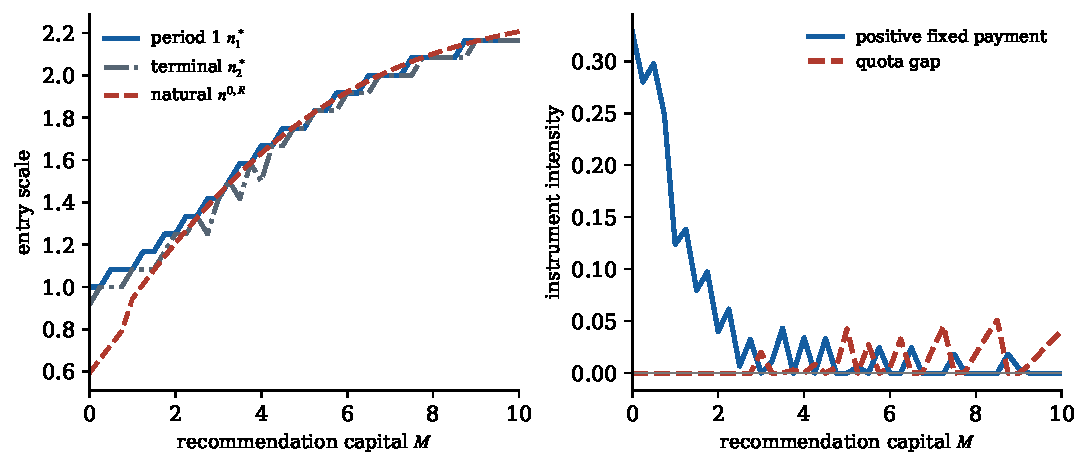
\includegraphics[width=0.98\textwidth]{figures/two_period_equilibrium_solution.pdf}
  \caption{两期均衡的向后归纳解}
  \label{fig:两期数值均衡}
  \begin{minipage}{0.94\textwidth}
    \footnotesize\raggedright
    注：固定$K=1.4$。左图比较第一期、终端期与按第一期最优收入分成计算的零支付
    自然进入；右图分别报告正固定支付和零支付配额缺口。全部曲线由同一组期内原语
    和状态转移求解，不使用单独拟合的目标进入函数。
  \end{minipage}
\end{figure}

\subsection{无限期均衡、工具边界与过渡路径}

实际治理环境的值函数迭代在223次Bellman更新后收敛，最终残差为
$8.47\times10^{-8}$。有符号转移与仅非负支持两种对照分别在224次和222次更新后
收敛，残差均低于$10^{-7}$。内部逻辑检查也通过：全网格最大激励强度为
$\max\zeta^R=3.460<c=5$，创作者努力问题保持严格凹；沿目标进入网格的最小实施
支付增量为$0.0355>0$；最优转移没有依靠把$K'$或$M'$截断在人工上界。

表\ref{tab:无限期参考状态}报告四个参考状态。早期状态$(0.5,0.5)$下，平台选择
$n=1.500$并支付$0.812$；随着两类资本积累，固定支付逐步降至接近零。在
$(3.5,8.5)$，最优进入$3.042$低于自然进入$3.088$，平台以零支付配额留下
$0.046$的缺口。收入分成没有机械地随成熟度单调变化，因为它同时协调创作者努力
与平台事后曝光；政策阶段的识别来自固定支付或配额，而不是强迫$s$承担所有调整。

\begin{table}[H]
  \centering
  \caption{无限期治理均衡的参考状态}
  \label{tab:无限期参考状态}
  \begin{tabular}{ccccccc}
    \toprule
    $K$ & $M$ & $n^G$ & $s^G$ & $n^{0,R}$ & 固定支付 & 配额缺口 \\
    \midrule
    0.5 & 0.5 & 1.500 & 0.3750 & 0.572 & 0.812 & 0.000 \\
    1.5 & 3.0 & 1.833 & 0.4375 & 1.588 & 0.233 & 0.000 \\
    2.5 & 6.0 & 2.458 & 0.3750 & 2.422 & 0.033 & 0.000 \\
    3.5 & 8.5 & 3.042 & 0.3750 & 3.088 & 0.000 & 0.046 \\
    \bottomrule
  \end{tabular}
\end{table}

图\ref{fig:无限期政策函数}把三种工具环境放在一起。有符号转移基准在
$\Psi^R<0$时可以收取进入费；仅非负支持的政策不能把进入降到自然规模以下；
“非负支持加配额”则在不计算负转移收入的情况下实施选择性准入。因此，三条曲线的
差异不是数值误差，而是工具集合不同所产生的经济差异。

\begin{figure}[H]
  \centering
  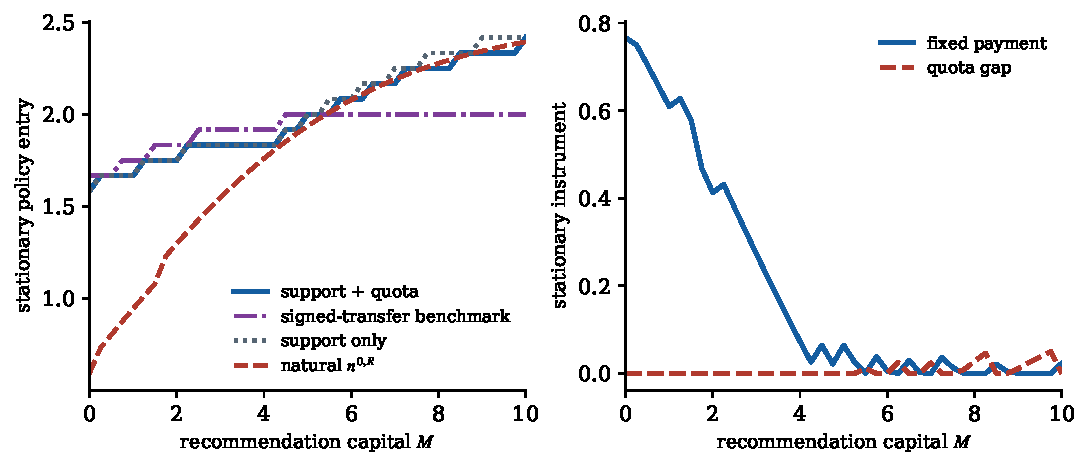
\includegraphics[width=0.98\textwidth]{figures/infinite_horizon_policy_solution.pdf}
  \caption{无限期平稳政策与工具集合}
  \label{fig:无限期政策函数}
  \begin{minipage}{0.94\textwidth}
    \footnotesize\raggedright
    注：固定$K=1.4$。有符号基准允许进入费；support only只允许统一非负固定支付；
    support $+$ quota在$\Psi^R<0$时令$I=0$并选择配额。右图报告实际治理环境的工具强度。
  \end{minipage}
\end{figure}

从$(K_0,M_0)=(0.2,0.2)$出发向前模拟60个经营批次，固定支付由$0.870$持续下降，
在零附近的离散行动之间短暂切换；第31期以后不再回到正支付，并持续使用小幅配额。
第60期达到$(K,M)=(3.974,8.396)$，进入约为$2.949$。图
\ref{fig:无限期转移路径}由同一平稳政策函数内生生成，未预先指定政策切换日期。

\begin{figure}[H]
  \centering
  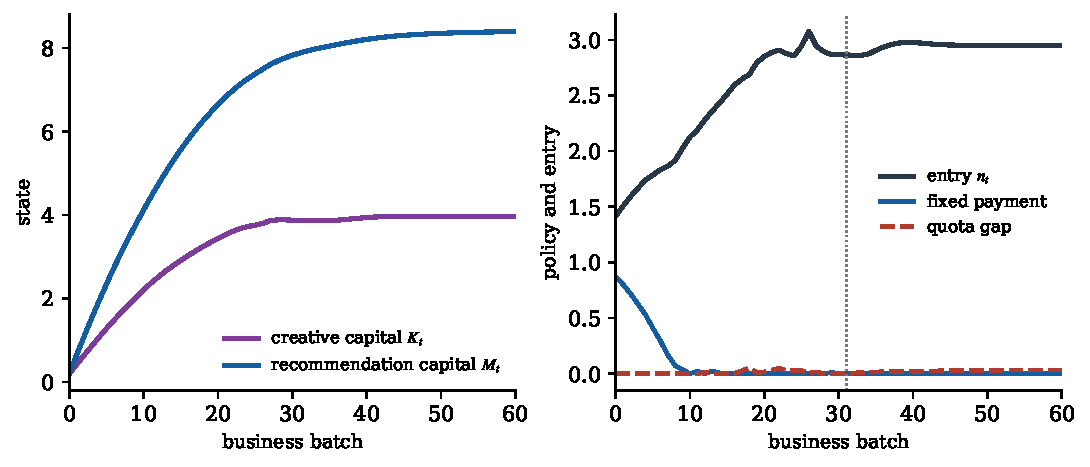
\includegraphics[width=0.98\textwidth]{figures/infinite_horizon_transition_solution.pdf}
  \caption{无限期均衡的内生状态与政策过渡}
  \label{fig:无限期转移路径}
  \begin{minipage}{0.94\textwidth}
    \footnotesize\raggedright
    注：左图为两类资本，右图为进入、固定支付和配额缺口。竖虚线表示模拟路径上
    正固定支付最后一次出现之后的首个批次；阈值附近的微小往返来自离散行动网格。
  \end{minipage}
\end{figure}

\subsection{敏感性、网格误差与可复现边界}

表\ref{tab:数值稳健性}改变折现、内容多样性、资本折旧和网格密度。所有情形均保留
“早期正支付、成熟状态存在配额缺口”的定性结论。较高$\beta$提高早期进入和支持，
因为平台更重视资本积累；更快折旧则降低长期状态。切换批次不必关于单个参数单调，
因为$K_t$和$M_t$同时改变自然进入、质量与政策函数。粗网格把永久切换推迟5个批次，
但参考状态的进入和支付差异较小，说明核心结论不依赖某一个网格点。

\begin{table}[H]
  \centering
  \scriptsize
  \caption{参数与网格敏感性}
  \label{tab:数值稳健性}
  \begin{tabular}{lcccccc}
    \toprule
    情形 & $\beta$ & $D$ & 初始进入 & 初始支付 & 成熟配额缺口 & 永久切换批次 \\
    \midrule
    基准细网格 & 0.92 & 0.875 & 1.500 & 0.812 & 0.046 & 31 \\
    粗网格 & 0.92 & 0.875 & 1.533 & 0.821 & 0.048 & 36 \\
    低折现 & 0.88 & 0.875 & 1.363 & 0.678 & 0.048 & 23 \\
    高折现 & 0.96 & 0.875 & 1.741 & 0.991 & 0.048 & 34 \\
    低多样性 & 0.92 & 0.775 & 1.474 & 0.777 & 0.040 & 27 \\
    高多样性 & 0.92 & 0.925 & 1.533 & 0.817 & 0.052 & 31 \\
    快折旧$(\delta_K,\delta_M)=(0.24,0.18)$ & 0.92 & 0.875 & 1.363 & 0.694 & 0.048 & 26 \\
    \bottomrule
  \end{tabular}
  \begin{minipage}{0.96\textwidth}
    \footnotesize\raggedright
    注：初始参考状态为$(K,M)=(0.5,0.5)$，成熟参考状态为$(3.5,8.5)$。粗网格为
    $21\times29$个状态、$37\times13$个行动；其余敏感性也在粗网格求解。
  \end{minipage}
\end{table}

全部计算由\path{scripts/solve_dynamic_equilibria.py}生成；参数、残差、参考状态和敏感性
结果保存在\path{output/computation/}，公开代码与数据的原始压缩包、校验值和使用边界
记录在\path{literature_recent_discrete_models/replication_code_sources/README.md}。这些
文件使数值结论可以复算，同时保留“算法借鉴”与“模型原创”的边界。
%%%
\section{可检验预测与经验设计}
\label{sec:emp}

\subsection{理论预测}
模型产生五组可以区分的经验预测。

第一，普惠固定支付或收入保底上升会扩大项目进入，但在推荐资本和内容构成不变时，
会降低单项目平均曝光、人工质量努力和变量收益。该稀释效应应当在题材同质度较高、
即$\vartheta(M,D)$较大的类别中更强；在内容差异较大的类别中，项目数增加造成的
有效拥堵较弱。

第二，当$v<r$时，收入分成对进入和质量努力呈倒U形，其转折点为
$s^\dagger=(v+r)/(2r)$。平台非分账价值$v$越高，转折点越靠右；若$v\geq r$，
在基准可行区间内收入分成对进入和努力不再出现下降段。

第三，推荐技术升级同时提高$\eta(M)$并降低$\vartheta(M,D)$时，应当提高新发布
和长尾项目的冷启动曝光、单项目有效绩效以及零补贴进入规模。其影响不仅体现为总
曝光增加，还应体现为相似项目之间的曝光挤出减弱。\citet{zhou2026wemm}报告的
生产部署结果与这一机制相容，但并不构成对本文结构参数或因果效应的直接估计。

第四，若式\eqref{eq:边际进入单交叉条件}与式\eqref{eq:边界穿越条件}成立，
推荐资本跨过$M^\dagger$以后，普惠补贴降至零而资格审核、项目申请制和定向扶持的
重要性上升。若观察到技术升级以后普惠补贴反而扩大，则表明匹配改善带来的当期
边际收益可能超过数据学习收益递减和拥堵成本，式\eqref{eq:原始分量充分条件}不成立。

第五，在随机学习扩展中，新增项目对后续决策准确率的影响应当在初始预测不确定性高、
且项目覆盖题材更分散时更强。若用冷启动样本量衡量$n_t$、用样本外预测误差的倒数
代理$\xi_t$，则式\eqref{eq:反馈信号精度}预言$n_t$与后续预测改善正相关，但
这一关系随$\xi_t$提高而减弱；同一规模下，较高的$D_t$应带来更大的改善。该预测
同时区分“多收集重复反馈”和“增加有效独立信息”。

\subsection{变量构造与识别思路}
经验研究可以使用“项目—平台—批次”面板。核心结果变量包括批次进入项目数、
单项目测试曝光、后续推荐曝光、有效观看或付费转化、人工精修投入以及项目退出。
固定支付$I_t$可以由制作补贴、保底金额或平台投资计划构造；收入分成$s_t$由合同
条款构造；平台推荐资本$M_t$可由明确的算法版本更新、冷启动识别准确率或上线前后
的匹配指标代理。在随机扩展中，$\mu_t$可由平台在批次开始时对题材或人群转化率的
预测构造，$\xi_t$可由预测区间宽度、后验方差或滚动样本外误差的倒数代理；二者
应当分别测量“平台预计什么会成功”和“平台对此有多确定”，不能合并为同一个准确率
指标。

内容多样性可以利用公开多模态表征模型生成项目向量。令标准化后的项目表示为$z_i$，
则批次多样性的一种可操作定义是
\begin{equation}
  D_t
  =1-\frac{2}{n_t(n_t-1)}
  \sum_{i<j}\frac{z_i^\top z_j}{\lVert z_i\rVert\lVert z_j\rVert}.
  \label{eq:经验多样性}
\end{equation}
WeMM-Embedding可以用于生成文本、封面和视频的统一表示\citep{zhou2026wemm}，
但经验部分应报告替代模型、不同向量维度和不同视频抽帧方式下的稳健性，避免把单一
表征模型的测量误差误认为经济效应。

若存在清晰的平台补贴调整或推荐系统升级时间，可以估计项目层面的事件研究：
\begin{equation}
  y_{ipt}
  =\alpha_i+\lambda_t
  +\sum_{\ell\neq-1}\beta_\ell
  \ind{t-T_p=\ell}
  +\gamma X_{ipt}+\varepsilon_{ipt},
  \label{eq:event-study}
\end{equation}
其中$T_p$为平台$p$的政策或技术变更时点，$y_{ipt}$依次取进入、曝光或绩效指标。
为检验语义拥堵机制，可以加入政策变量与$D_t$或平均相似度的交互项。由于补贴和算法
升级通常会响应既有增长趋势、内容质量和监管环境，简单的前后比较不能解释为因果效应；
至少需要检验事件前趋势，并利用分批上线、资格边界或其他外生实施差异加强识别。

\section{结论与适用边界}
\label{sec:conclusion}

生成式人工智能对内容市场的影响不止是一次生产率冲击。它降低部分创作任务的成本，
扩大能够进入市场的项目集合，同时把平台的核心约束推向内容发现、注意力配置、审核
和跨期学习。本文以AI短剧为主要应用，构造一个生成式内容平台的动态模型，将固定
支付、收入分成、人工质量努力和事后推荐置于同一时序中。模型的核心对象是新增项目
的动态边际价值：新增项目既产生当期经营与爆款发现价值，也积累创作资本和推荐资本，
但还会加剧注意力拥堵、筛选成本和激励稀释。

这一框架给出的主要解释是“稀缺性的迁移”。推荐资本较低时，平台尚不了解新的题材、
团队和用户群，扩大项目试验具有较高的数据与发现价值，普惠式支持因而可能最优。
随着自然进入增加和推荐资本成熟，新增相似项目提供的学习价值下降，平台的稀缺资源
转为测试流量、审核能力和高质量人工精修。此时，将补贴简单降至零仍可能带来过多
自然进入，平台需要通过资格审核、项目申请制或定向扶持实施更低的目标规模。生成式
人工智能因此未必削弱平台的中介作用；在内容供给变得廉价以后，平台的识别和治理
能力反而可能更重要。

随机学习扩展为这一机制补充了信息基础。平台对潜在内容---用户匹配状态的认知由
后验均值$\mu_t$和后验精度$\xi_t$概括，项目数量、多样性与有效绩效共同决定
反馈信号精度。平台据此面对一个受控马尔可夫决策问题：新增项目不仅改变当期利润和
创作资本，也通过更有信息量的后验分布改善未来政策适配。当这一信息边际价值随既有
精度递减时，确定性成熟阈值推广为$\xi^\dagger(K,\mu)$；当凹性或单交叉失败时，
随机阈值也可能不存在。因而，贝叶斯更新提供的是可检验的状态转移，而不是保证政策
必然转换的数学装饰。

上述结论是关于利润最大化平台的正向预测，而不是“选择性准入必然提高社会福利”的
规范判断。平台治理研究已经表明，平台的收费方式和竞争激励可能使准入、推荐或质量
标准相对社会最优过松或过严\citep{teh2022governance}。本文尚未显式写入用户剩余、
创作者长期职业选择、平台间竞争和内容表达多样性的独立社会价值，因此
$M>M^\dagger$只意味着统一非负支付无法实施平台自己的目标进入规模。若要评价监管
政策，还需要把平台目标与社会规划者目标分开，并纳入错误淘汰、创新多样性和创作者
剩余。

模型也具有明确边界。它是单平台的局部均衡模型，将用户规模和潜在项目池视为给定，
并令每期进入的创作者主要进行当期优化；它没有处理创作者多归属、基础模型定价、
版权责任、平台自制内容以及用户对AI标签的偏好。数值部分求解的是一组经过数据矩
约束的部分校准均衡，而不是结构估计；其中短视频类别数据只约束多样性，不能识别
现实AI短剧合同或福利参数。因而，本文最适合解释那些由平台集中分发、依赖推荐冷启动、存在标准化
扶持或分成并能从项目反馈中学习的生成式内容市场。AI短剧满足这些条件，是优先的
经验检验场景；向其他内容类别外推时，应首先验证上述制度条件是否成立。

\section{附录}
\label{sec:appendix}

\begin{appendices}
\section{符号表}
\begin{itemize}
  \item $K_t$：创作资本；$M_t$：平台推荐资本；$\tau$：外生生成式人工智能技术水平。
  \item $I_t$：单位项目固定支付；$s_t$：创作者收入分成；$\Lambda(s_t)=v+(1-s_t)r$：平台单位绩效剩余价值。
  \item $n_t$：进入项目规模；$k_{i,t}$：项目固定制作成本；$F_k$：固定成本分布。
  \item $e_{i,t}$：人工质量努力；$q_{i,t}$：内容质量；$x_{i,t}$：推荐曝光；$Y_{i,t}$：有效绩效。
  \item $\eta(M_t)$：多模态识别与用户匹配效率；$D_t$：内容多样性；$\vartheta(M_t,D_t)$：有效注意力重叠。
  \item $\mathcal B(n_t)$：当期爆款发现价值；$C_N(n_t)$：筛选、版权核验与审核成本。
  \item $G_K,G_M$：创作资本和推荐资本积累函数；$\delta_K,\delta_M$：相应折旧率；$\beta$：平台折现因子。
  \item $\Psi^R$：实施目标进入规模所需的固定支付；$n^{0,R}$：零补贴自然进入规模；$n^d$：有符号转移支付辅助基准中的动态目标进入规模。
  \item $\Omega_1$与$\overline\Omega$：两期和无限期模型中的动态边际进入价值；$M^\dagger$：普惠支持转向选择性准入的推荐资本阈值。
  \item $V_t(K_t,M_t)$与$V(K,M)$：有限期和无限期平台价值函数。
  \item $\theta_t$：随机扩展中的潜在内容---用户匹配状态；$\mu_t$与$\xi_t$：其后验均值与后验精度。
  \item $\mathcal T_t$：当期项目反馈的有效信号精度；$Q_B$：贝叶斯更新诱导的受控马尔可夫转移核。
  \item $W(K,\mu,\xi)$：随机学习扩展中的平台价值函数；$\Omega^B$与$\xi^\dagger(K,\mu)$：随机动态边际进入价值与后验精度阈值。
\end{itemize}

\section{离散时期的解释}
本文的一期对应一个合同和内容批次完成全部经营环节的时间窗口。窗口长度可以在经验
应用中按月、季度或一次平台扶持计划的结算周期确定。期内推荐可以包含多轮实时排序，
模型只要求这些高频决策在批次结束时形成可汇总的曝光、绩效与数据反馈。因而，离散
时间不是关于平台只能在固定日期更新算法的技术断言，而是对高频经营活动的经济聚合。
这一解释也避免把WeMM-Embedding的两阶段训练流程误认为本文的两个经济时期。

\section{数值均衡算法与复现检查}

算法\ref{alg:两期向后归纳}先在终端期逐状态求最大值，再用双线性插值评价第一期
行动产生的非网格下一期状态。创作者侧变量不进入额外行动维度，而是在每个候选
$(n,s)$下由命题\ref{prop:多模态期内均衡}解析代回。

\begin{algorithm}[H]
  \caption{两期均衡的向后归纳}
  \label{alg:两期向后归纳}
  \begin{algorithmic}[1]
    \Require 状态网格$\mathcal G_K\times\mathcal G_M$，行动网格$\mathcal G_n\times\mathcal G_s$
    \For{每个状态$(K,M)$和行动$(n,s)$}
      \State 计算$e^R,q^R,Y^R,S^R,g^R,\Psi^R$和治理利润$\Pi^G$
      \State 计算下一状态$(K',M')$及其插值索引与权重
    \EndFor
    \For{每个终端状态$(K,M)$}
      \State $V_2(K,M)\gets\max_{n,s}\Pi^G(K,M,n,s)$并保存最优行动
    \EndFor
    \For{每个第一期状态$(K,M)$}
      \State 以双线性插值得到$\widehat V_2(K',M')$
      \State $V_1(K,M)\gets\max_{n,s}\{\Pi^G+\beta\widehat V_2(K',M')\}$并保存最优行动
    \EndFor
  \end{algorithmic}
\end{algorithm}

算法\ref{alg:无限期VFI}对无限期Bellman算子进行值函数迭代。收敛以后再额外进行
一次完整Bellman更新；报告的残差是该次更新与已收敛价值函数的上确界距离，而不是
只报告相邻两次迭代看起来相近。

\begin{algorithm}[H]
  \caption{无限期平稳马尔可夫均衡的值函数迭代}
  \label{alg:无限期VFI}
  \begin{algorithmic}[1]
    \Require 预计算的$\Pi^G(K,M,n,s)$、下一状态插值索引与权重；容差$\varepsilon=10^{-7}$
    \State 初始化$V^{(0)}(K,M)=0$，令$j=0$
    \Repeat
      \For{每个状态$(K,M)$}
        \State $V^{(j+1)}(K,M)\gets\max_{n,s}\{\Pi^G+\beta\widehat V^{(j)}(K',M')\}$
        \State 保存实现最大值的$(n^{(j+1)},s^{(j+1)})$
      \EndFor
      \State $d_j\gets\lVert V^{(j+1)}-V^{(j)}\rVert_\infty$，$j\gets j+1$
    \Until{$d_{j-1}<\varepsilon$}
    \State 再应用一次Bellman算子，报告残差$\lVert\mathcal TV^{(j)}-V^{(j)}\rVert_\infty$
    \State 从给定$(K_0,M_0)$按平稳政策和式\eqref{eq:数值状态转移}向前模拟
  \end{algorithmic}
\end{algorithm}

基准求解的三项必要内部检查为：$\max\zeta^R<c$、沿$n$网格的
$\Delta\Psi^R>0$以及转移不撞击状态空间上界。它们分别排除创作者努力非凹、目标
进入表示失去单调性和数值结果由边界截断制造三类逻辑错误。敏感性分析另外改变状态
与行动网格，核验政策阶段转换不是某个离散点的产物。
\end{appendices}

\bibliographystyle{apalike}
\bibliography{references}

\end{document}
